\section{zesto-cache.h File Reference}
\label{zesto-cache_8h}\index{zesto-cache.h@{zesto-cache.h}}


This graph shows which files directly or indirectly include this file:\nopagebreak
\begin{figure}[H]
\begin{center}
\leavevmode
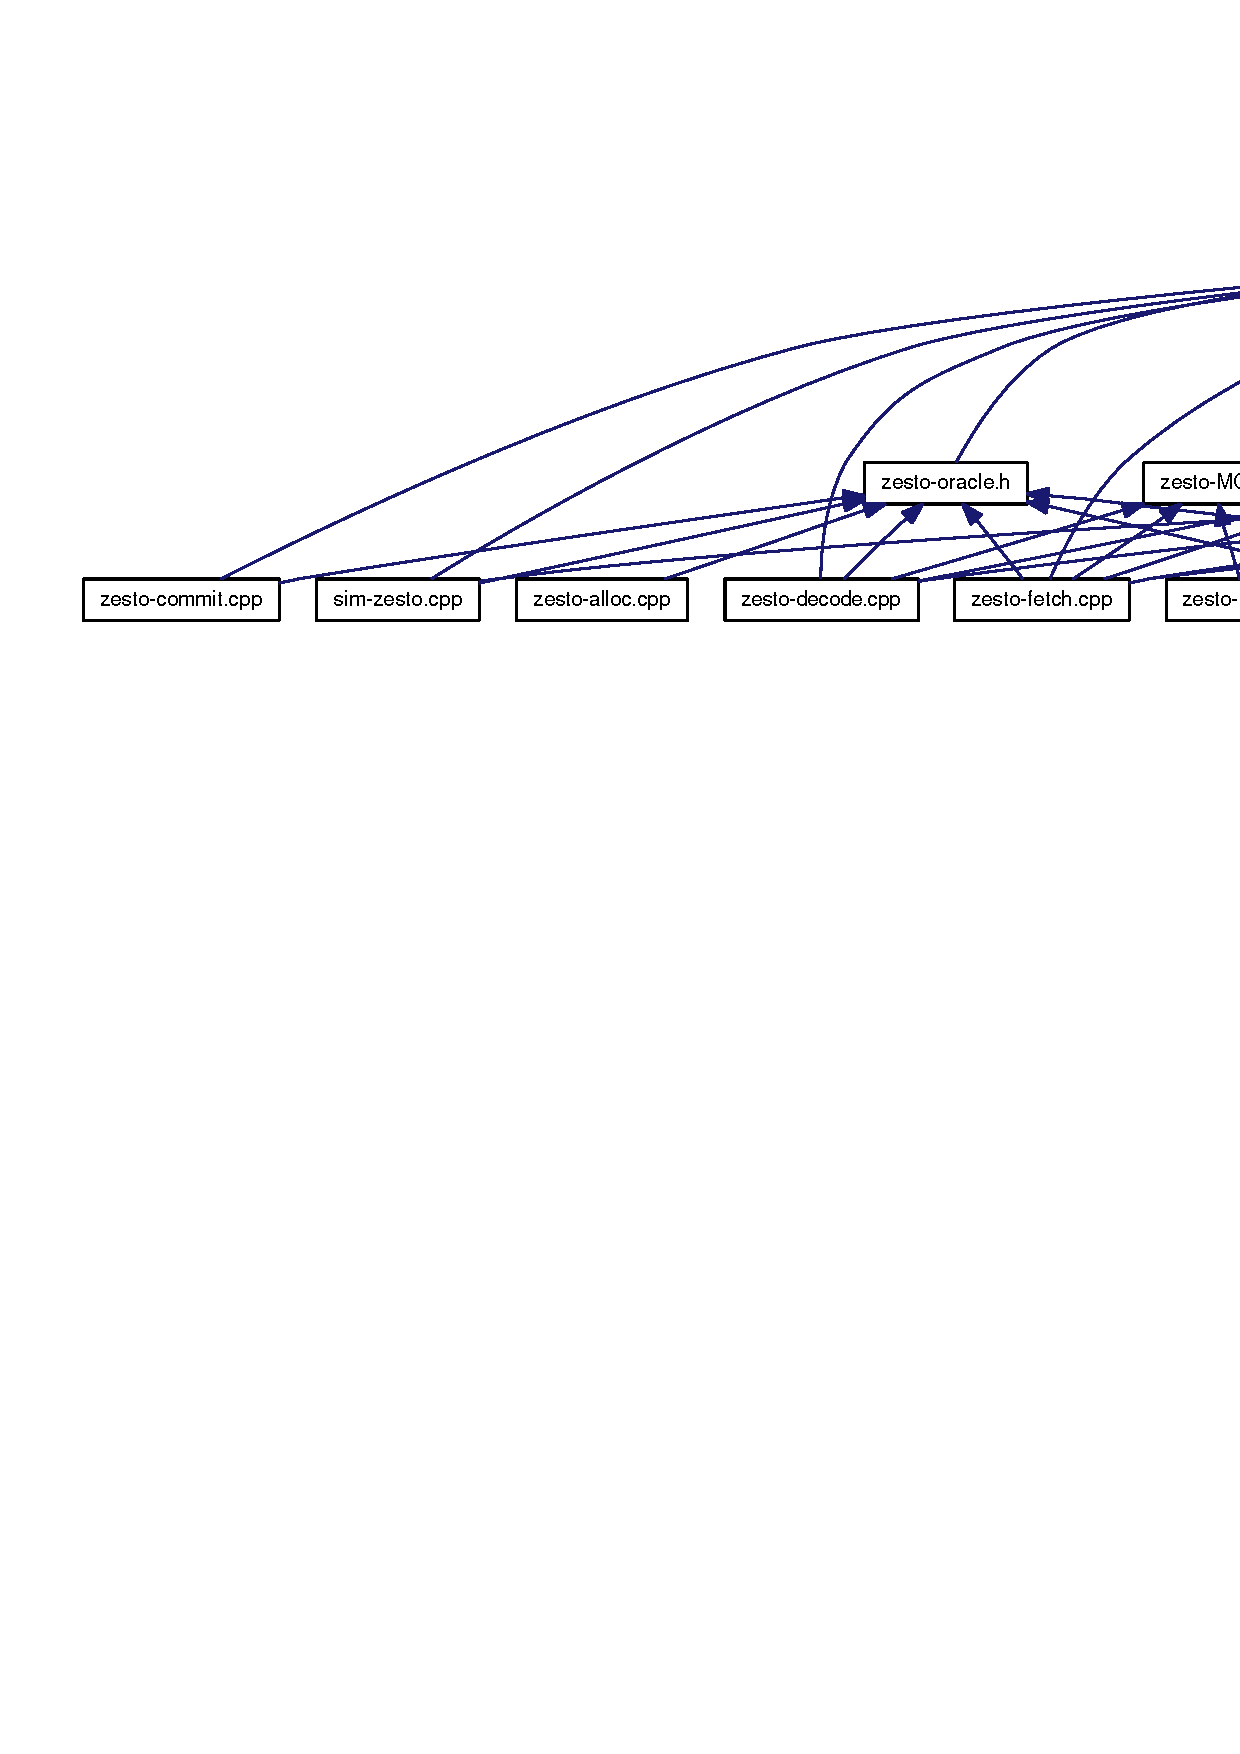
\includegraphics[width=420pt]{zesto-cache_8h__dep__incl}
\end{center}
\end{figure}
\subsection*{Classes}
\begin{CompactItemize}
\item 
struct {\bf cache\_\-line\_\-t}
\item 
struct {\bf cache\_\-action\_\-t}
\item 
struct {\bf cache\_\-fill\_\-t}
\item 
struct {\bf prefetch\_\-buffer\_\-t}
\item 
struct {\bf prefetch\_\-filter\_\-t}
\item 
struct {\bf bus\_\-t}
\item 
struct {\bf cache\_\-t}
\item 
struct {\bf cache\_\-t::cache\_\-t::PFF\_\-t}
\end{CompactItemize}
\subsection*{Defines}
\begin{CompactItemize}
\item 
\#define {\bf NO\_\-MSHR}~(-1)
\item 
\#define {\bf BIG\_\-LATENCY}~99999
\item 
\#define {\bf CACHE\_\-STAT}(x)~\{if(!cp $\rightarrow$ frozen) \{x\}\}
\item 
\#define {\bf GET\_\-BANK}(x)~(((x)$>$$>$cp $\rightarrow$ bank\_\-shift) \& cp $\rightarrow$ bank\_\-mask)
\item 
\#define {\bf GET\_\-MSHR\_\-BANK}(x)~(((x)$>$$>$cp $\rightarrow$ bank\_\-shift) \& cp $\rightarrow$ MSHR\_\-mask)
\item 
\#define {\bf cache\_\-fatal}(msg, retval)
\item 
\#define {\bf cache\_\-assert}(cond, retval)
\end{CompactItemize}
\subsection*{Enumerations}
\begin{CompactItemize}
\item 
enum {\bf cache\_\-command} \{ \par
{\bf CACHE\_\-NOP}, 
{\bf CACHE\_\-READ}, 
{\bf CACHE\_\-WRITE}, 
{\bf CACHE\_\-WRITEBACK}, 
\par
{\bf CACHE\_\-PREFETCH}, 
{\bf REFRESH}, 
{\bf CACHE\_\-NOP}, 
{\bf CACHE\_\-READ}, 
\par
{\bf CACHE\_\-WRITE}, 
{\bf CACHE\_\-WRITEBACK}, 
{\bf CACHE\_\-PREFETCH}, 
{\bf REFRESH}, 
\par
{\bf INVALIDATE}, 
{\bf FWD\_\-DIRTY}, 
{\bf READ\_\-RESPONSE}, 
{\bf WRITE\_\-RESPONSE}, 
\par
{\bf ACK}
 \}
\item 
enum {\bf repl\_\-policy\_\-t} \{ \par
{\bf REPLACE\_\-LRU}, 
{\bf REPLACE\_\-MRU}, 
{\bf REPLACE\_\-RANDOM}, 
{\bf REPLACE\_\-NMRU}, 
\par
{\bf REPLACE\_\-PLRU}, 
{\bf REPLACE\_\-CLOCK}, 
{\bf REPLACE\_\-LRU}, 
{\bf REPLACE\_\-MRU}, 
\par
{\bf REPLACE\_\-RANDOM}, 
{\bf REPLACE\_\-NMRU}, 
{\bf REPLACE\_\-PLRU}, 
{\bf REPLACE\_\-CLOCK}
 \}
\item 
enum {\bf alloc\_\-policy\_\-t} \{ {\bf WRITE\_\-ALLOC}, 
{\bf NO\_\-WRITE\_\-ALLOC}, 
{\bf WRITE\_\-ALLOC}, 
{\bf NO\_\-WRITE\_\-ALLOC}
 \}
\item 
enum {\bf write\_\-policy\_\-t} \{ {\bf WRITE\_\-THROUGH}, 
{\bf WRITE\_\-BACK}, 
{\bf WRITE\_\-THROUGH}, 
{\bf WRITE\_\-BACK}
 \}
\item 
enum {\bf read\_\-only\_\-t} \{ {\bf CACHE\_\-READWRITE}, 
{\bf CACHE\_\-READONLY}, 
{\bf CACHE\_\-READWRITE}, 
{\bf CACHE\_\-READONLY}
 \}
\item 
enum {\bf coherence\_\-state} \{ {\bf MOD}, 
{\bf EXC}, 
{\bf SHR}, 
{\bf INV}
 \}
\item 
enum {\bf PF\_\-state\_\-t} \{ {\bf PF\_\-REFRAIN}, 
{\bf PF\_\-OK}
 \}
\end{CompactItemize}
\subsection*{Functions}
\begin{CompactItemize}
\item 
struct {\bf cache\_\-t} $\ast$ {\bf cache\_\-create} (struct {\bf core\_\-t} $\ast$const core, const char $\ast$const name, const bool read\_\-only, const int sets, const int assoc, const int linesize, const char rp, const char ap, const char wp, const char wc, const int banks, const int bank\_\-width, const int latency, const int WBB\_\-size, const int MSHR\_\-size, const int MSHR\_\-banked, struct {\bf cache\_\-t} $\ast$const next\_\-level\_\-cache, struct {\bf bus\_\-t} $\ast$const bus\_\-next)
\item 
struct {\bf cache\_\-t} $\ast$ {\bf cache\_\-create\_\-llc} (struct {\bf core\_\-t} $\ast$const core, const char $\ast$const name, const bool read\_\-only, const int sets, const int assoc, const int linesize, const char rp, const char ap, const char wp, const char wc, const int banks, const int bank\_\-width, const int latency, const int WBB\_\-size, const int MSHR\_\-size, const int MSHR\_\-banked, const int begin\_\-index, const int end\_\-index, struct {\bf cache\_\-t} $\ast$const next\_\-level\_\-cache, struct {\bf bus\_\-t} $\ast$const bus\_\-next)
\item 
void {\bf cache\_\-reg\_\-stats} (struct {\bf stat\_\-sdb\_\-t} $\ast$const sdb, const struct {\bf core\_\-t} $\ast$const core, struct {\bf cache\_\-t} $\ast$const cp)
\item 
void {\bf LLC\_\-reg\_\-stats} (struct {\bf stat\_\-sdb\_\-t} $\ast$const sdb, struct {\bf cache\_\-t} $\ast$const cp)
\item 
void {\bf cache\_\-reset\_\-stats} (struct {\bf cache\_\-t} $\ast$const cp)
\item 
void {\bf prefetch\_\-buffer\_\-create} (struct {\bf cache\_\-t} $\ast$const cp, const int num\_\-entries)
\item 
void {\bf prefetch\_\-filter\_\-create} (struct {\bf cache\_\-t} $\ast$const cp, const int num\_\-entries, const int reset\_\-interval)
\item 
void {\bf cache\_\-process} (struct {\bf cache\_\-t} $\ast$const cp)
\item 
void {\bf cache\_\-process\_\-llc} (struct {\bf cache\_\-t} $\ast$const cp)
\item 
struct {\bf cache\_\-line\_\-t} $\ast$ {\bf cache\_\-is\_\-hit} (struct {\bf cache\_\-t} $\ast$const cp, const enum {\bf cache\_\-command} cmd, const {\bf md\_\-paddr\_\-t} addr, struct {\bf core\_\-t} $\ast$const core)
\item 
struct {\bf cache\_\-line\_\-t} $\ast$ {\bf cache\_\-is\_\-hit\_\-llc} (struct {\bf cache\_\-t} $\ast$const cp, const enum {\bf cache\_\-command} cmd, const {\bf md\_\-paddr\_\-t} addr, struct {\bf core\_\-t} $\ast$const core)
\item 
void {\bf cache\_\-insert\_\-block} (struct {\bf cache\_\-t} $\ast$const cp, const enum {\bf cache\_\-command} cmd, const {\bf md\_\-paddr\_\-t} addr, struct {\bf core\_\-t} $\ast$const core)
\item 
struct {\bf cache\_\-line\_\-t} $\ast$ {\bf cache\_\-invalidate} (struct {\bf cache\_\-t} $\ast$const cp, const {\bf md\_\-paddr\_\-t} addr, {\bf core\_\-t} $\ast$const core)
\item 
void {\bf cache\_\-insert\_\-block\_\-llc} (struct {\bf cache\_\-t} $\ast$const cp, const enum {\bf cache\_\-command} cmd, const {\bf md\_\-paddr\_\-t} addr, struct {\bf core\_\-t} $\ast$const core)
\item 
struct {\bf cache\_\-line\_\-t} $\ast$ {\bf cache\_\-get\_\-evictee} (struct {\bf cache\_\-t} $\ast$const cp, const {\bf md\_\-paddr\_\-t} addr, struct {\bf core\_\-t} $\ast$const core)
\item 
struct {\bf cache\_\-line\_\-t} $\ast$ {\bf cache\_\-get\_\-evictee\_\-llc} (struct {\bf cache\_\-t} $\ast$const cp, const {\bf md\_\-paddr\_\-t} addr, struct {\bf core\_\-t} $\ast$const core)
\item 
int {\bf cache\_\-enqueuable} (const struct {\bf cache\_\-t} $\ast$const cp, const int thread\_\-id, const {\bf md\_\-paddr\_\-t} addr)
\item 
int {\bf cache\_\-enqueuable\_\-llc} (const struct {\bf cache\_\-t} $\ast$const cp, const int thread\_\-id, const {\bf md\_\-paddr\_\-t} addr)
\item 
void {\bf cache\_\-enqueue} (struct {\bf core\_\-t} $\ast$const core, struct {\bf cache\_\-t} $\ast$const cp, struct {\bf cache\_\-t} $\ast$const prev\_\-cp, const enum {\bf cache\_\-command} cmd, const int thread\_\-id, const {\bf md\_\-addr\_\-t} PC, const {\bf md\_\-paddr\_\-t} addr, const {\bf seq\_\-t} action\_\-id, const int MSHR\_\-bank, const int MSHR\_\-index, void $\ast$const op, void($\ast$const cb)(void $\ast$), void($\ast$const miss\_\-cb)(void $\ast$, int), bool($\ast$const translated\_\-cb)(void $\ast$, {\bf seq\_\-t}), {\bf seq\_\-t}($\ast$const get\_\-action\_\-id)(void $\ast$))
\item 
void {\bf cache\_\-enqueue\_\-llc} (struct {\bf core\_\-t} $\ast$const core, struct {\bf cache\_\-t} $\ast$const cp, struct {\bf cache\_\-t} $\ast$const prev\_\-cp, const enum {\bf cache\_\-command} cmd, const int thread\_\-id, const {\bf md\_\-addr\_\-t} PC, const {\bf md\_\-paddr\_\-t} addr, const {\bf seq\_\-t} action\_\-id, const int MSHR\_\-bank, const int MSHR\_\-index, void $\ast$const op, void($\ast$const cb)(void $\ast$), void($\ast$const miss\_\-cb)(void $\ast$, int), bool($\ast$const translated\_\-cb)(void $\ast$, {\bf seq\_\-t}), {\bf seq\_\-t}($\ast$const get\_\-action\_\-id)(void $\ast$))
\item 
void {\bf fill\_\-arrived} (struct {\bf cache\_\-t} $\ast$const cp, const int MSHR\_\-bank, const int MSHR\_\-index)
\item 
void {\bf fill\_\-arrived\_\-llc} (struct {\bf cache\_\-t} $\ast$const cp, unsigned long long int address)
\item 
void {\bf step\_\-core\_\-PF\_\-controllers} (struct {\bf core\_\-t} $\ast$const core)
\item 
void {\bf prefetch\_\-core\_\-caches} (struct {\bf core\_\-t} $\ast$const core)
\item 
void {\bf step\_\-LLC\_\-PF\_\-controller} (struct {\bf uncore\_\-t} $\ast$const uncore)
\item 
void {\bf prefetch\_\-LLC} (struct {\bf uncore\_\-t} $\ast$const uncore)
\item 
void {\bf cache\_\-freeze\_\-stats} (struct {\bf core\_\-t} $\ast$const core)
\item 
struct {\bf bus\_\-t} $\ast$ {\bf bus\_\-create} (const char $\ast$const name, const int width, const int ratio)
\item 
void {\bf bus\_\-reg\_\-stats} (struct {\bf stat\_\-sdb\_\-t} $\ast$const sdb, struct {\bf core\_\-t} $\ast$const core, struct {\bf bus\_\-t} $\ast$const bus)
\item 
int {\bf bus\_\-free} (const struct {\bf bus\_\-t} $\ast$const bus)
\item 
void {\bf bus\_\-use} (struct {\bf bus\_\-t} $\ast$const bus, const int transfer\_\-size, const int prefetch)
\end{CompactItemize}


\subsection{Define Documentation}
\index{zesto-cache.h@{zesto-cache.h}!BIG\_\-LATENCY@{BIG\_\-LATENCY}}
\index{BIG\_\-LATENCY@{BIG\_\-LATENCY}!zesto-cache.h@{zesto-cache.h}}
\subsubsection[{BIG\_\-LATENCY}]{\setlength{\rightskip}{0pt plus 5cm}\#define BIG\_\-LATENCY~99999}\label{zesto-cache_8h_8d2ff015ca2239311fb6533186242f9e}




Definition at line 87 of file zesto-cache.h.\index{zesto-cache.h@{zesto-cache.h}!cache\_\-assert@{cache\_\-assert}}
\index{cache\_\-assert@{cache\_\-assert}!zesto-cache.h@{zesto-cache.h}}
\subsubsection[{cache\_\-assert}]{\setlength{\rightskip}{0pt plus 5cm}\#define cache\_\-assert(cond, \/  retval)}\label{zesto-cache_8h_353f3b46190659b8825fac08a8eb7938}


\textbf{Value:}

\begin{Code}\begin{verbatim}{ \
  if(!(cond)) { \
    fprintf(stderr,"assertion failed (%s,%d:%s): ",__FILE__,__LINE__,cp->name); \
    fprintf(stderr,"%s\n",#cond); \
    return (retval); \
  } \
}
\end{verbatim}
\end{Code}


Definition at line 515 of file zesto-cache.h.\index{zesto-cache.h@{zesto-cache.h}!cache\_\-fatal@{cache\_\-fatal}}
\index{cache\_\-fatal@{cache\_\-fatal}!zesto-cache.h@{zesto-cache.h}}
\subsubsection[{cache\_\-fatal}]{\setlength{\rightskip}{0pt plus 5cm}\#define cache\_\-fatal(msg, \/  retval)}\label{zesto-cache_8h_49d297d9664074880fe05898300c0389}


\textbf{Value:}

\begin{Code}\begin{verbatim}{ \
  fprintf(stderr,"fatal (%s,%d:%s): ",__FILE__,__LINE__,cp->name); \
  fprintf(stderr,"%s\n",msg); \
  return (retval); \
}
\end{verbatim}
\end{Code}


Definition at line 503 of file zesto-cache.h.\index{zesto-cache.h@{zesto-cache.h}!CACHE\_\-STAT@{CACHE\_\-STAT}}
\index{CACHE\_\-STAT@{CACHE\_\-STAT}!zesto-cache.h@{zesto-cache.h}}
\subsubsection[{CACHE\_\-STAT}]{\setlength{\rightskip}{0pt plus 5cm}\#define CACHE\_\-STAT(x)~\{if(!cp $\rightarrow$ frozen) \{x\}\}}\label{zesto-cache_8h_0b5d48674769c2e561375e0710d91169}




Definition at line 89 of file zesto-cache.h.\index{zesto-cache.h@{zesto-cache.h}!GET\_\-BANK@{GET\_\-BANK}}
\index{GET\_\-BANK@{GET\_\-BANK}!zesto-cache.h@{zesto-cache.h}}
\subsubsection[{GET\_\-BANK}]{\setlength{\rightskip}{0pt plus 5cm}\#define GET\_\-BANK(x)~(((x)$>$$>$cp $\rightarrow$ bank\_\-shift) \& cp $\rightarrow$ bank\_\-mask)}\label{zesto-cache_8h_1567854259cffa374f9ef7ba763e2586}




Definition at line 91 of file zesto-cache.h.\index{zesto-cache.h@{zesto-cache.h}!GET\_\-MSHR\_\-BANK@{GET\_\-MSHR\_\-BANK}}
\index{GET\_\-MSHR\_\-BANK@{GET\_\-MSHR\_\-BANK}!zesto-cache.h@{zesto-cache.h}}
\subsubsection[{GET\_\-MSHR\_\-BANK}]{\setlength{\rightskip}{0pt plus 5cm}\#define GET\_\-MSHR\_\-BANK(x)~(((x)$>$$>$cp $\rightarrow$ bank\_\-shift) \& cp $\rightarrow$ MSHR\_\-mask)}\label{zesto-cache_8h_088d13f1f3edc2a38285413565b6a11e}




Definition at line 92 of file zesto-cache.h.\index{zesto-cache.h@{zesto-cache.h}!NO\_\-MSHR@{NO\_\-MSHR}}
\index{NO\_\-MSHR@{NO\_\-MSHR}!zesto-cache.h@{zesto-cache.h}}
\subsubsection[{NO\_\-MSHR}]{\setlength{\rightskip}{0pt plus 5cm}\#define NO\_\-MSHR~(-1)}\label{zesto-cache_8h_47d3ac5bd49bbf1ff15859f38059ac97}




Definition at line 83 of file zesto-cache.h.

\subsection{Enumeration Type Documentation}
\index{zesto-cache.h@{zesto-cache.h}!alloc\_\-policy\_\-t@{alloc\_\-policy\_\-t}}
\index{alloc\_\-policy\_\-t@{alloc\_\-policy\_\-t}!zesto-cache.h@{zesto-cache.h}}
\subsubsection[{alloc\_\-policy\_\-t}]{\setlength{\rightskip}{0pt plus 5cm}enum {\bf alloc\_\-policy\_\-t}}\label{zesto-cache_8h_143ef0e79644952fb702e2fc59039a97}


\begin{Desc}
\item[Enumerator: ]\par
\begin{description}
\index{WRITE\_\-ALLOC@{WRITE\_\-ALLOC}!zesto-cache.h@{zesto-cache.h}}\index{zesto-cache.h@{zesto-cache.h}!WRITE\_\-ALLOC@{WRITE\_\-ALLOC}}\item[{\em 
WRITE\_\-ALLOC\label{zesto-cache_8h_143ef0e79644952fb702e2fc59039a97707810d553b893dc4eec7d37bfa1723a}
}]\index{NO\_\-WRITE\_\-ALLOC@{NO\_\-WRITE\_\-ALLOC}!zesto-cache.h@{zesto-cache.h}}\index{zesto-cache.h@{zesto-cache.h}!NO\_\-WRITE\_\-ALLOC@{NO\_\-WRITE\_\-ALLOC}}\item[{\em 
NO\_\-WRITE\_\-ALLOC\label{zesto-cache_8h_143ef0e79644952fb702e2fc59039a97e8f5a75c8ca1933266708cd57262ed8f}
}]\index{WRITE\_\-ALLOC@{WRITE\_\-ALLOC}!zesto-cache.h@{zesto-cache.h}}\index{zesto-cache.h@{zesto-cache.h}!WRITE\_\-ALLOC@{WRITE\_\-ALLOC}}\item[{\em 
WRITE\_\-ALLOC\label{zesto-cache_8h_143ef0e79644952fb702e2fc59039a97707810d553b893dc4eec7d37bfa1723a}
}]\index{NO\_\-WRITE\_\-ALLOC@{NO\_\-WRITE\_\-ALLOC}!zesto-cache.h@{zesto-cache.h}}\index{zesto-cache.h@{zesto-cache.h}!NO\_\-WRITE\_\-ALLOC@{NO\_\-WRITE\_\-ALLOC}}\item[{\em 
NO\_\-WRITE\_\-ALLOC\label{zesto-cache_8h_143ef0e79644952fb702e2fc59039a97e8f5a75c8ca1933266708cd57262ed8f}
}]\end{description}
\end{Desc}



Definition at line 103 of file zesto-cache.h.\index{zesto-cache.h@{zesto-cache.h}!cache\_\-command@{cache\_\-command}}
\index{cache\_\-command@{cache\_\-command}!zesto-cache.h@{zesto-cache.h}}
\subsubsection[{cache\_\-command}]{\setlength{\rightskip}{0pt plus 5cm}enum {\bf cache\_\-command}}\label{zesto-cache_8h_aa2f5ac205a00e5df606ccf951edb255}


\begin{Desc}
\item[Enumerator: ]\par
\begin{description}
\index{CACHE\_\-NOP@{CACHE\_\-NOP}!zesto-cache.h@{zesto-cache.h}}\index{zesto-cache.h@{zesto-cache.h}!CACHE\_\-NOP@{CACHE\_\-NOP}}\item[{\em 
CACHE\_\-NOP\label{zesto-cache_8h_aa2f5ac205a00e5df606ccf951edb2553db1607181aed3c809ffeec523d5d9e6}
}]\index{CACHE\_\-READ@{CACHE\_\-READ}!zesto-cache.h@{zesto-cache.h}}\index{zesto-cache.h@{zesto-cache.h}!CACHE\_\-READ@{CACHE\_\-READ}}\item[{\em 
CACHE\_\-READ\label{zesto-cache_8h_aa2f5ac205a00e5df606ccf951edb255a614c7f88fbcfcc7dc4e5e9fd697f585}
}]\index{CACHE\_\-WRITE@{CACHE\_\-WRITE}!zesto-cache.h@{zesto-cache.h}}\index{zesto-cache.h@{zesto-cache.h}!CACHE\_\-WRITE@{CACHE\_\-WRITE}}\item[{\em 
CACHE\_\-WRITE\label{zesto-cache_8h_aa2f5ac205a00e5df606ccf951edb255f31232fbf9e45b41922cf68b09a4a201}
}]\index{CACHE\_\-WRITEBACK@{CACHE\_\-WRITEBACK}!zesto-cache.h@{zesto-cache.h}}\index{zesto-cache.h@{zesto-cache.h}!CACHE\_\-WRITEBACK@{CACHE\_\-WRITEBACK}}\item[{\em 
CACHE\_\-WRITEBACK\label{zesto-cache_8h_aa2f5ac205a00e5df606ccf951edb25532d220872fec4028b8b25e094c84837c}
}]\index{CACHE\_\-PREFETCH@{CACHE\_\-PREFETCH}!zesto-cache.h@{zesto-cache.h}}\index{zesto-cache.h@{zesto-cache.h}!CACHE\_\-PREFETCH@{CACHE\_\-PREFETCH}}\item[{\em 
CACHE\_\-PREFETCH\label{zesto-cache_8h_aa2f5ac205a00e5df606ccf951edb25537348416545a4253a253b1a4371e6ccf}
}]\index{REFRESH@{REFRESH}!zesto-cache.h@{zesto-cache.h}}\index{zesto-cache.h@{zesto-cache.h}!REFRESH@{REFRESH}}\item[{\em 
REFRESH\label{zesto-cache_8h_aa2f5ac205a00e5df606ccf951edb2551418c4911c72f0c5ae1eed401facb41a}
}]\index{CACHE\_\-NOP@{CACHE\_\-NOP}!zesto-cache.h@{zesto-cache.h}}\index{zesto-cache.h@{zesto-cache.h}!CACHE\_\-NOP@{CACHE\_\-NOP}}\item[{\em 
CACHE\_\-NOP\label{zesto-cache_8h_aa2f5ac205a00e5df606ccf951edb2553db1607181aed3c809ffeec523d5d9e6}
}]\index{CACHE\_\-READ@{CACHE\_\-READ}!zesto-cache.h@{zesto-cache.h}}\index{zesto-cache.h@{zesto-cache.h}!CACHE\_\-READ@{CACHE\_\-READ}}\item[{\em 
CACHE\_\-READ\label{zesto-cache_8h_aa2f5ac205a00e5df606ccf951edb255a614c7f88fbcfcc7dc4e5e9fd697f585}
}]\index{CACHE\_\-WRITE@{CACHE\_\-WRITE}!zesto-cache.h@{zesto-cache.h}}\index{zesto-cache.h@{zesto-cache.h}!CACHE\_\-WRITE@{CACHE\_\-WRITE}}\item[{\em 
CACHE\_\-WRITE\label{zesto-cache_8h_aa2f5ac205a00e5df606ccf951edb255f31232fbf9e45b41922cf68b09a4a201}
}]\index{CACHE\_\-WRITEBACK@{CACHE\_\-WRITEBACK}!zesto-cache.h@{zesto-cache.h}}\index{zesto-cache.h@{zesto-cache.h}!CACHE\_\-WRITEBACK@{CACHE\_\-WRITEBACK}}\item[{\em 
CACHE\_\-WRITEBACK\label{zesto-cache_8h_aa2f5ac205a00e5df606ccf951edb25532d220872fec4028b8b25e094c84837c}
}]\index{CACHE\_\-PREFETCH@{CACHE\_\-PREFETCH}!zesto-cache.h@{zesto-cache.h}}\index{zesto-cache.h@{zesto-cache.h}!CACHE\_\-PREFETCH@{CACHE\_\-PREFETCH}}\item[{\em 
CACHE\_\-PREFETCH\label{zesto-cache_8h_aa2f5ac205a00e5df606ccf951edb25537348416545a4253a253b1a4371e6ccf}
}]\index{REFRESH@{REFRESH}!zesto-cache.h@{zesto-cache.h}}\index{zesto-cache.h@{zesto-cache.h}!REFRESH@{REFRESH}}\item[{\em 
REFRESH\label{zesto-cache_8h_aa2f5ac205a00e5df606ccf951edb2551418c4911c72f0c5ae1eed401facb41a}
}]\index{INVALIDATE@{INVALIDATE}!zesto-cache.h@{zesto-cache.h}}\index{zesto-cache.h@{zesto-cache.h}!INVALIDATE@{INVALIDATE}}\item[{\em 
INVALIDATE\label{zesto-cache_8h_aa2f5ac205a00e5df606ccf951edb255db971f7bfd0eb4ce85796906d5141d4e}
}]\index{FWD\_\-DIRTY@{FWD\_\-DIRTY}!zesto-cache.h@{zesto-cache.h}}\index{zesto-cache.h@{zesto-cache.h}!FWD\_\-DIRTY@{FWD\_\-DIRTY}}\item[{\em 
FWD\_\-DIRTY\label{zesto-cache_8h_aa2f5ac205a00e5df606ccf951edb2555f1076a8e7a1de7c448809baf13d00d5}
}]\index{READ\_\-RESPONSE@{READ\_\-RESPONSE}!zesto-cache.h@{zesto-cache.h}}\index{zesto-cache.h@{zesto-cache.h}!READ\_\-RESPONSE@{READ\_\-RESPONSE}}\item[{\em 
READ\_\-RESPONSE\label{zesto-cache_8h_aa2f5ac205a00e5df606ccf951edb255faf9ed0bebace3689903e00b134650f6}
}]\index{WRITE\_\-RESPONSE@{WRITE\_\-RESPONSE}!zesto-cache.h@{zesto-cache.h}}\index{zesto-cache.h@{zesto-cache.h}!WRITE\_\-RESPONSE@{WRITE\_\-RESPONSE}}\item[{\em 
WRITE\_\-RESPONSE\label{zesto-cache_8h_aa2f5ac205a00e5df606ccf951edb25521da40a5b2a4e0349b0ee23721dabd52}
}]\index{ACK@{ACK}!zesto-cache.h@{zesto-cache.h}}\index{zesto-cache.h@{zesto-cache.h}!ACK@{ACK}}\item[{\em 
ACK\label{zesto-cache_8h_aa2f5ac205a00e5df606ccf951edb25541246e9c8691b7e33bc79b345e06b48e}
}]\end{description}
\end{Desc}



Definition at line 96 of file zesto-cache.h.\index{zesto-cache.h@{zesto-cache.h}!coherence\_\-state@{coherence\_\-state}}
\index{coherence\_\-state@{coherence\_\-state}!zesto-cache.h@{zesto-cache.h}}
\subsubsection[{coherence\_\-state}]{\setlength{\rightskip}{0pt plus 5cm}enum {\bf coherence\_\-state}}\label{zesto-cache_8h_1783fb5ddbc5c1cdba69734881c803f9}


\begin{Desc}
\item[Enumerator: ]\par
\begin{description}
\index{MOD@{MOD}!zesto-cache.h@{zesto-cache.h}}\index{zesto-cache.h@{zesto-cache.h}!MOD@{MOD}}\item[{\em 
MOD\label{zesto-cache_8h_1783fb5ddbc5c1cdba69734881c803f9140fcc89db148e5975f1486e794675ba}
}]\index{EXC@{EXC}!zesto-cache.h@{zesto-cache.h}}\index{zesto-cache.h@{zesto-cache.h}!EXC@{EXC}}\item[{\em 
EXC\label{zesto-cache_8h_1783fb5ddbc5c1cdba69734881c803f9c7ce650289a5b15320b2026f08d9d4ec}
}]\index{SHR@{SHR}!zesto-cache.h@{zesto-cache.h}}\index{zesto-cache.h@{zesto-cache.h}!SHR@{SHR}}\item[{\em 
SHR\label{zesto-cache_8h_1783fb5ddbc5c1cdba69734881c803f9dea444991c90042dd6201f2a83ad309d}
}]\index{INV@{INV}!zesto-cache.h@{zesto-cache.h}}\index{zesto-cache.h@{zesto-cache.h}!INV@{INV}}\item[{\em 
INV\label{zesto-cache_8h_1783fb5ddbc5c1cdba69734881c803f9003b741848d7128e25831a8376672700}
}]\end{description}
\end{Desc}



Definition at line 106 of file zesto-cache.h.\index{zesto-cache.h@{zesto-cache.h}!PF\_\-state\_\-t@{PF\_\-state\_\-t}}
\index{PF\_\-state\_\-t@{PF\_\-state\_\-t}!zesto-cache.h@{zesto-cache.h}}
\subsubsection[{PF\_\-state\_\-t}]{\setlength{\rightskip}{0pt plus 5cm}enum {\bf PF\_\-state\_\-t}}\label{zesto-cache_8h_86b849e99f917fca61d33518c5954b37}


\begin{Desc}
\item[Enumerator: ]\par
\begin{description}
\index{PF\_\-REFRAIN@{PF\_\-REFRAIN}!zesto-cache.h@{zesto-cache.h}}\index{zesto-cache.h@{zesto-cache.h}!PF\_\-REFRAIN@{PF\_\-REFRAIN}}\item[{\em 
PF\_\-REFRAIN\label{zesto-cache_8h_86b849e99f917fca61d33518c5954b37a1d05c179b0a4d19bff06a82e1fbb341}
}]\index{PF\_\-OK@{PF\_\-OK}!zesto-cache.h@{zesto-cache.h}}\index{zesto-cache.h@{zesto-cache.h}!PF\_\-OK@{PF\_\-OK}}\item[{\em 
PF\_\-OK\label{zesto-cache_8h_86b849e99f917fca61d33518c5954b37f842d0e9d4f1635527e54dfe37cc9fe2}
}]\end{description}
\end{Desc}



Definition at line 108 of file zesto-cache.h.\index{zesto-cache.h@{zesto-cache.h}!read\_\-only\_\-t@{read\_\-only\_\-t}}
\index{read\_\-only\_\-t@{read\_\-only\_\-t}!zesto-cache.h@{zesto-cache.h}}
\subsubsection[{read\_\-only\_\-t}]{\setlength{\rightskip}{0pt plus 5cm}enum {\bf read\_\-only\_\-t}}\label{zesto-cache_8h_6cb413fabed99a64137321b4c9779aa1}


\begin{Desc}
\item[Enumerator: ]\par
\begin{description}
\index{CACHE\_\-READWRITE@{CACHE\_\-READWRITE}!zesto-cache.h@{zesto-cache.h}}\index{zesto-cache.h@{zesto-cache.h}!CACHE\_\-READWRITE@{CACHE\_\-READWRITE}}\item[{\em 
CACHE\_\-READWRITE\label{zesto-cache_8h_6cb413fabed99a64137321b4c9779aa1d22ad1643074e988a0af228750966eb4}
}]\index{CACHE\_\-READONLY@{CACHE\_\-READONLY}!zesto-cache.h@{zesto-cache.h}}\index{zesto-cache.h@{zesto-cache.h}!CACHE\_\-READONLY@{CACHE\_\-READONLY}}\item[{\em 
CACHE\_\-READONLY\label{zesto-cache_8h_6cb413fabed99a64137321b4c9779aa139ba0426a3586969e21ebb44709e8de3}
}]\index{CACHE\_\-READWRITE@{CACHE\_\-READWRITE}!zesto-cache.h@{zesto-cache.h}}\index{zesto-cache.h@{zesto-cache.h}!CACHE\_\-READWRITE@{CACHE\_\-READWRITE}}\item[{\em 
CACHE\_\-READWRITE\label{zesto-cache_8h_6cb413fabed99a64137321b4c9779aa1d22ad1643074e988a0af228750966eb4}
}]\index{CACHE\_\-READONLY@{CACHE\_\-READONLY}!zesto-cache.h@{zesto-cache.h}}\index{zesto-cache.h@{zesto-cache.h}!CACHE\_\-READONLY@{CACHE\_\-READONLY}}\item[{\em 
CACHE\_\-READONLY\label{zesto-cache_8h_6cb413fabed99a64137321b4c9779aa139ba0426a3586969e21ebb44709e8de3}
}]\end{description}
\end{Desc}



Definition at line 105 of file zesto-cache.h.\index{zesto-cache.h@{zesto-cache.h}!repl\_\-policy\_\-t@{repl\_\-policy\_\-t}}
\index{repl\_\-policy\_\-t@{repl\_\-policy\_\-t}!zesto-cache.h@{zesto-cache.h}}
\subsubsection[{repl\_\-policy\_\-t}]{\setlength{\rightskip}{0pt plus 5cm}enum {\bf repl\_\-policy\_\-t}}\label{zesto-cache_8h_3c03a1f892e597e168b382b4d02ce5ee}


\begin{Desc}
\item[Enumerator: ]\par
\begin{description}
\index{REPLACE\_\-LRU@{REPLACE\_\-LRU}!zesto-cache.h@{zesto-cache.h}}\index{zesto-cache.h@{zesto-cache.h}!REPLACE\_\-LRU@{REPLACE\_\-LRU}}\item[{\em 
REPLACE\_\-LRU\label{zesto-cache_8h_3c03a1f892e597e168b382b4d02ce5eebf7bce8ff5e2ff3b783d8e6ac096d3af}
}]\index{REPLACE\_\-MRU@{REPLACE\_\-MRU}!zesto-cache.h@{zesto-cache.h}}\index{zesto-cache.h@{zesto-cache.h}!REPLACE\_\-MRU@{REPLACE\_\-MRU}}\item[{\em 
REPLACE\_\-MRU\label{zesto-cache_8h_3c03a1f892e597e168b382b4d02ce5ee339e2ef8aa3980cc6df60991809f13b9}
}]\index{REPLACE\_\-RANDOM@{REPLACE\_\-RANDOM}!zesto-cache.h@{zesto-cache.h}}\index{zesto-cache.h@{zesto-cache.h}!REPLACE\_\-RANDOM@{REPLACE\_\-RANDOM}}\item[{\em 
REPLACE\_\-RANDOM\label{zesto-cache_8h_3c03a1f892e597e168b382b4d02ce5eeca558b7c4cf12cb0cde222a828ddf992}
}]\index{REPLACE\_\-NMRU@{REPLACE\_\-NMRU}!zesto-cache.h@{zesto-cache.h}}\index{zesto-cache.h@{zesto-cache.h}!REPLACE\_\-NMRU@{REPLACE\_\-NMRU}}\item[{\em 
REPLACE\_\-NMRU\label{zesto-cache_8h_3c03a1f892e597e168b382b4d02ce5ee8dd71f35db07407c9e4246fa359b6cbf}
}]\index{REPLACE\_\-PLRU@{REPLACE\_\-PLRU}!zesto-cache.h@{zesto-cache.h}}\index{zesto-cache.h@{zesto-cache.h}!REPLACE\_\-PLRU@{REPLACE\_\-PLRU}}\item[{\em 
REPLACE\_\-PLRU\label{zesto-cache_8h_3c03a1f892e597e168b382b4d02ce5eef0eb4dfc64984fa952f4e789caabdbe2}
}]\index{REPLACE\_\-CLOCK@{REPLACE\_\-CLOCK}!zesto-cache.h@{zesto-cache.h}}\index{zesto-cache.h@{zesto-cache.h}!REPLACE\_\-CLOCK@{REPLACE\_\-CLOCK}}\item[{\em 
REPLACE\_\-CLOCK\label{zesto-cache_8h_3c03a1f892e597e168b382b4d02ce5eee07aa96a0e515c0df5c762eded6ba9cb}
}]\index{REPLACE\_\-LRU@{REPLACE\_\-LRU}!zesto-cache.h@{zesto-cache.h}}\index{zesto-cache.h@{zesto-cache.h}!REPLACE\_\-LRU@{REPLACE\_\-LRU}}\item[{\em 
REPLACE\_\-LRU\label{zesto-cache_8h_3c03a1f892e597e168b382b4d02ce5eebf7bce8ff5e2ff3b783d8e6ac096d3af}
}]\index{REPLACE\_\-MRU@{REPLACE\_\-MRU}!zesto-cache.h@{zesto-cache.h}}\index{zesto-cache.h@{zesto-cache.h}!REPLACE\_\-MRU@{REPLACE\_\-MRU}}\item[{\em 
REPLACE\_\-MRU\label{zesto-cache_8h_3c03a1f892e597e168b382b4d02ce5ee339e2ef8aa3980cc6df60991809f13b9}
}]\index{REPLACE\_\-RANDOM@{REPLACE\_\-RANDOM}!zesto-cache.h@{zesto-cache.h}}\index{zesto-cache.h@{zesto-cache.h}!REPLACE\_\-RANDOM@{REPLACE\_\-RANDOM}}\item[{\em 
REPLACE\_\-RANDOM\label{zesto-cache_8h_3c03a1f892e597e168b382b4d02ce5eeca558b7c4cf12cb0cde222a828ddf992}
}]\index{REPLACE\_\-NMRU@{REPLACE\_\-NMRU}!zesto-cache.h@{zesto-cache.h}}\index{zesto-cache.h@{zesto-cache.h}!REPLACE\_\-NMRU@{REPLACE\_\-NMRU}}\item[{\em 
REPLACE\_\-NMRU\label{zesto-cache_8h_3c03a1f892e597e168b382b4d02ce5ee8dd71f35db07407c9e4246fa359b6cbf}
}]\index{REPLACE\_\-PLRU@{REPLACE\_\-PLRU}!zesto-cache.h@{zesto-cache.h}}\index{zesto-cache.h@{zesto-cache.h}!REPLACE\_\-PLRU@{REPLACE\_\-PLRU}}\item[{\em 
REPLACE\_\-PLRU\label{zesto-cache_8h_3c03a1f892e597e168b382b4d02ce5eef0eb4dfc64984fa952f4e789caabdbe2}
}]\index{REPLACE\_\-CLOCK@{REPLACE\_\-CLOCK}!zesto-cache.h@{zesto-cache.h}}\index{zesto-cache.h@{zesto-cache.h}!REPLACE\_\-CLOCK@{REPLACE\_\-CLOCK}}\item[{\em 
REPLACE\_\-CLOCK\label{zesto-cache_8h_3c03a1f892e597e168b382b4d02ce5eee07aa96a0e515c0df5c762eded6ba9cb}
}]\end{description}
\end{Desc}



Definition at line 102 of file zesto-cache.h.\index{zesto-cache.h@{zesto-cache.h}!write\_\-policy\_\-t@{write\_\-policy\_\-t}}
\index{write\_\-policy\_\-t@{write\_\-policy\_\-t}!zesto-cache.h@{zesto-cache.h}}
\subsubsection[{write\_\-policy\_\-t}]{\setlength{\rightskip}{0pt plus 5cm}enum {\bf write\_\-policy\_\-t}}\label{zesto-cache_8h_2b253745ab48e94316d34a6e5e424f03}


\begin{Desc}
\item[Enumerator: ]\par
\begin{description}
\index{WRITE\_\-THROUGH@{WRITE\_\-THROUGH}!zesto-cache.h@{zesto-cache.h}}\index{zesto-cache.h@{zesto-cache.h}!WRITE\_\-THROUGH@{WRITE\_\-THROUGH}}\item[{\em 
WRITE\_\-THROUGH\label{zesto-cache_8h_2b253745ab48e94316d34a6e5e424f03283caacb51a1aef132663bf4ca1d481b}
}]\index{WRITE\_\-BACK@{WRITE\_\-BACK}!zesto-cache.h@{zesto-cache.h}}\index{zesto-cache.h@{zesto-cache.h}!WRITE\_\-BACK@{WRITE\_\-BACK}}\item[{\em 
WRITE\_\-BACK\label{zesto-cache_8h_2b253745ab48e94316d34a6e5e424f030ba8fedce0a574dd30058959e8e50ad8}
}]\index{WRITE\_\-THROUGH@{WRITE\_\-THROUGH}!zesto-cache.h@{zesto-cache.h}}\index{zesto-cache.h@{zesto-cache.h}!WRITE\_\-THROUGH@{WRITE\_\-THROUGH}}\item[{\em 
WRITE\_\-THROUGH\label{zesto-cache_8h_2b253745ab48e94316d34a6e5e424f03283caacb51a1aef132663bf4ca1d481b}
}]\index{WRITE\_\-BACK@{WRITE\_\-BACK}!zesto-cache.h@{zesto-cache.h}}\index{zesto-cache.h@{zesto-cache.h}!WRITE\_\-BACK@{WRITE\_\-BACK}}\item[{\em 
WRITE\_\-BACK\label{zesto-cache_8h_2b253745ab48e94316d34a6e5e424f030ba8fedce0a574dd30058959e8e50ad8}
}]\end{description}
\end{Desc}



Definition at line 104 of file zesto-cache.h.

\subsection{Function Documentation}
\index{zesto-cache.h@{zesto-cache.h}!bus\_\-create@{bus\_\-create}}
\index{bus\_\-create@{bus\_\-create}!zesto-cache.h@{zesto-cache.h}}
\subsubsection[{bus\_\-create}]{\setlength{\rightskip}{0pt plus 5cm}struct {\bf bus\_\-t}$\ast$ bus\_\-create (const char $\ast$const  {\em name}, \/  const int {\em width}, \/  const int {\em ratio})\hspace{0.3cm}{\tt  [read]}}\label{zesto-cache_8h_cf58fdfdf1939cc2b0b05b50ac0eedd8}




Definition at line 2465 of file config/zesto-cache.cpp.

References fatal(), bus\_\-t::name, bus\_\-t::ratio, and bus\_\-t::width.

Referenced by core\_\-exec\_\-DPM\_\-t::core\_\-exec\_\-DPM\_\-t(), core\_\-exec\_\-STM\_\-t::core\_\-exec\_\-STM\_\-t(), and uncore\_\-t::uncore\_\-t().

Here is the caller graph for this function:\nopagebreak
\begin{figure}[H]
\begin{center}
\leavevmode
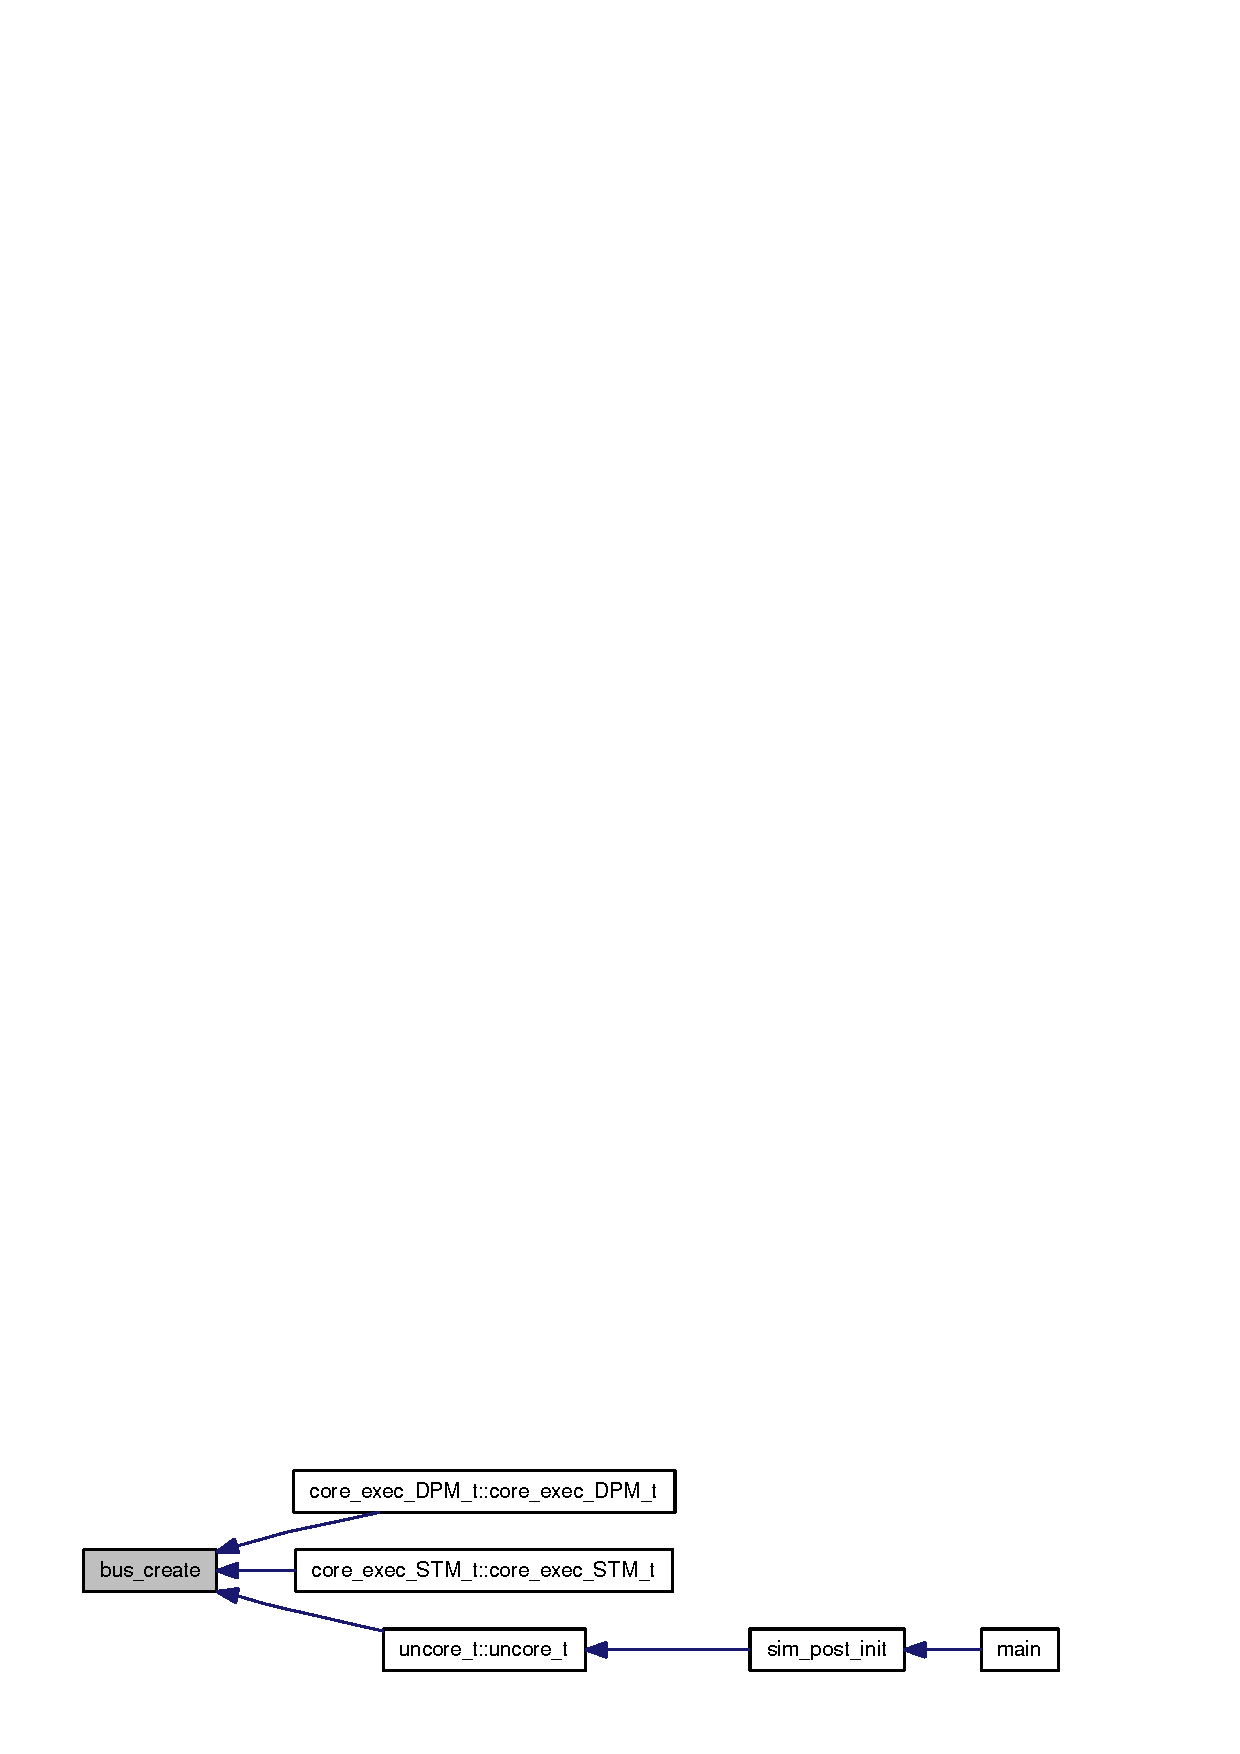
\includegraphics[width=256pt]{zesto-cache_8h_cf58fdfdf1939cc2b0b05b50ac0eedd8_icgraph}
\end{center}
\end{figure}
\index{zesto-cache.h@{zesto-cache.h}!bus\_\-free@{bus\_\-free}}
\index{bus\_\-free@{bus\_\-free}!zesto-cache.h@{zesto-cache.h}}
\subsubsection[{bus\_\-free}]{\setlength{\rightskip}{0pt plus 5cm}int bus\_\-free (const struct {\bf bus\_\-t} $\ast$const  {\em bus})}\label{zesto-cache_8h_24292dcf41327971f03a4c7150cbdf28}




Definition at line 2518 of file config/zesto-cache.cpp.

References bus\_\-t::ratio, sim\_\-cycle, and bus\_\-t::when\_\-available.

Referenced by cache\_\-process(), and cache\_\-process\_\-llc().

Here is the caller graph for this function:\nopagebreak
\begin{figure}[H]
\begin{center}
\leavevmode
\includegraphics[width=211pt]{zesto-cache_8h_24292dcf41327971f03a4c7150cbdf28_icgraph}
\end{center}
\end{figure}
\index{zesto-cache.h@{zesto-cache.h}!bus\_\-reg\_\-stats@{bus\_\-reg\_\-stats}}
\index{bus\_\-reg\_\-stats@{bus\_\-reg\_\-stats}!zesto-cache.h@{zesto-cache.h}}
\subsubsection[{bus\_\-reg\_\-stats}]{\setlength{\rightskip}{0pt plus 5cm}void bus\_\-reg\_\-stats (struct {\bf stat\_\-sdb\_\-t} $\ast$const  {\em sdb}, \/  struct {\bf core\_\-t} $\ast$const  {\em core}, \/  struct {\bf bus\_\-t} $\ast$const  {\em bus})}\label{zesto-cache_8h_22d7e9c4a1a2031601e5a3ad3694768c}




Definition at line 2479 of file config/zesto-cache.cpp.

References bus\_\-t::accesses, core\_\-t::current\_\-thread, thread\_\-t::id, bus\_\-t::name, bus\_\-t::prefetch\_\-utilization, bus\_\-t::stat, stat\_\-reg\_\-counter, stat\_\-reg\_\-formula(), and bus\_\-t::utilization.

Referenced by core\_\-exec\_\-STM\_\-t::reg\_\-stats(), and uncore\_\-t::uncore\_\-reg\_\-stats().

Here is the caller graph for this function:\nopagebreak
\begin{figure}[H]
\begin{center}
\leavevmode
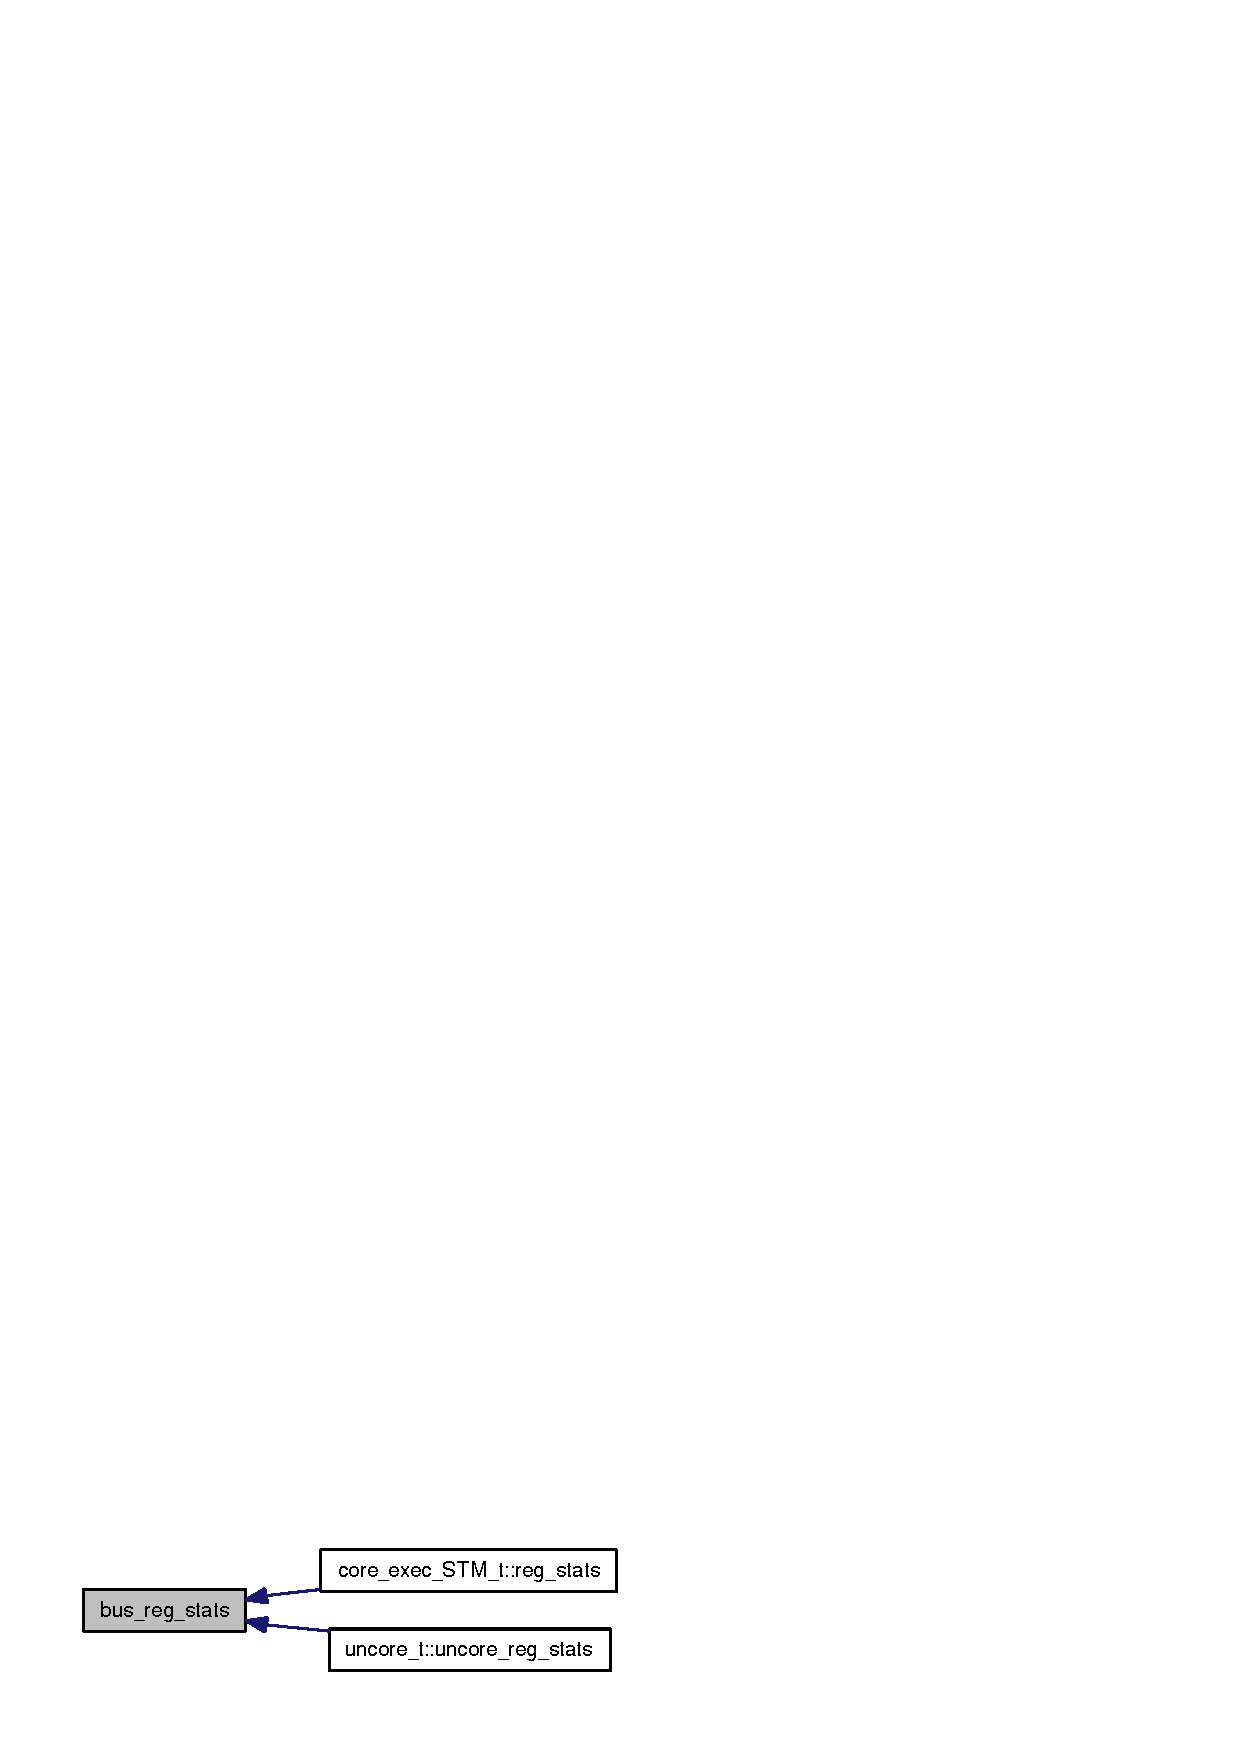
\includegraphics[width=150pt]{zesto-cache_8h_22d7e9c4a1a2031601e5a3ad3694768c_icgraph}
\end{center}
\end{figure}
\index{zesto-cache.h@{zesto-cache.h}!bus\_\-use@{bus\_\-use}}
\index{bus\_\-use@{bus\_\-use}!zesto-cache.h@{zesto-cache.h}}
\subsubsection[{bus\_\-use}]{\setlength{\rightskip}{0pt plus 5cm}void bus\_\-use (struct {\bf bus\_\-t} $\ast$const  {\em bus}, \/  const int {\em transfer\_\-size}, \/  const int {\em prefetch})}\label{zesto-cache_8h_cb6440bff7b9405665cbae0d836630f3}




Definition at line 2529 of file config/zesto-cache.cpp.

References bus\_\-t::accesses, bus\_\-t::prefetch\_\-utilization, bus\_\-t::ratio, sim\_\-cycle, bus\_\-t::stat, bus\_\-t::utilization, bus\_\-t::when\_\-available, and bus\_\-t::width.

Referenced by cache\_\-process(), and cache\_\-process\_\-llc().

Here is the caller graph for this function:\nopagebreak
\begin{figure}[H]
\begin{center}
\leavevmode
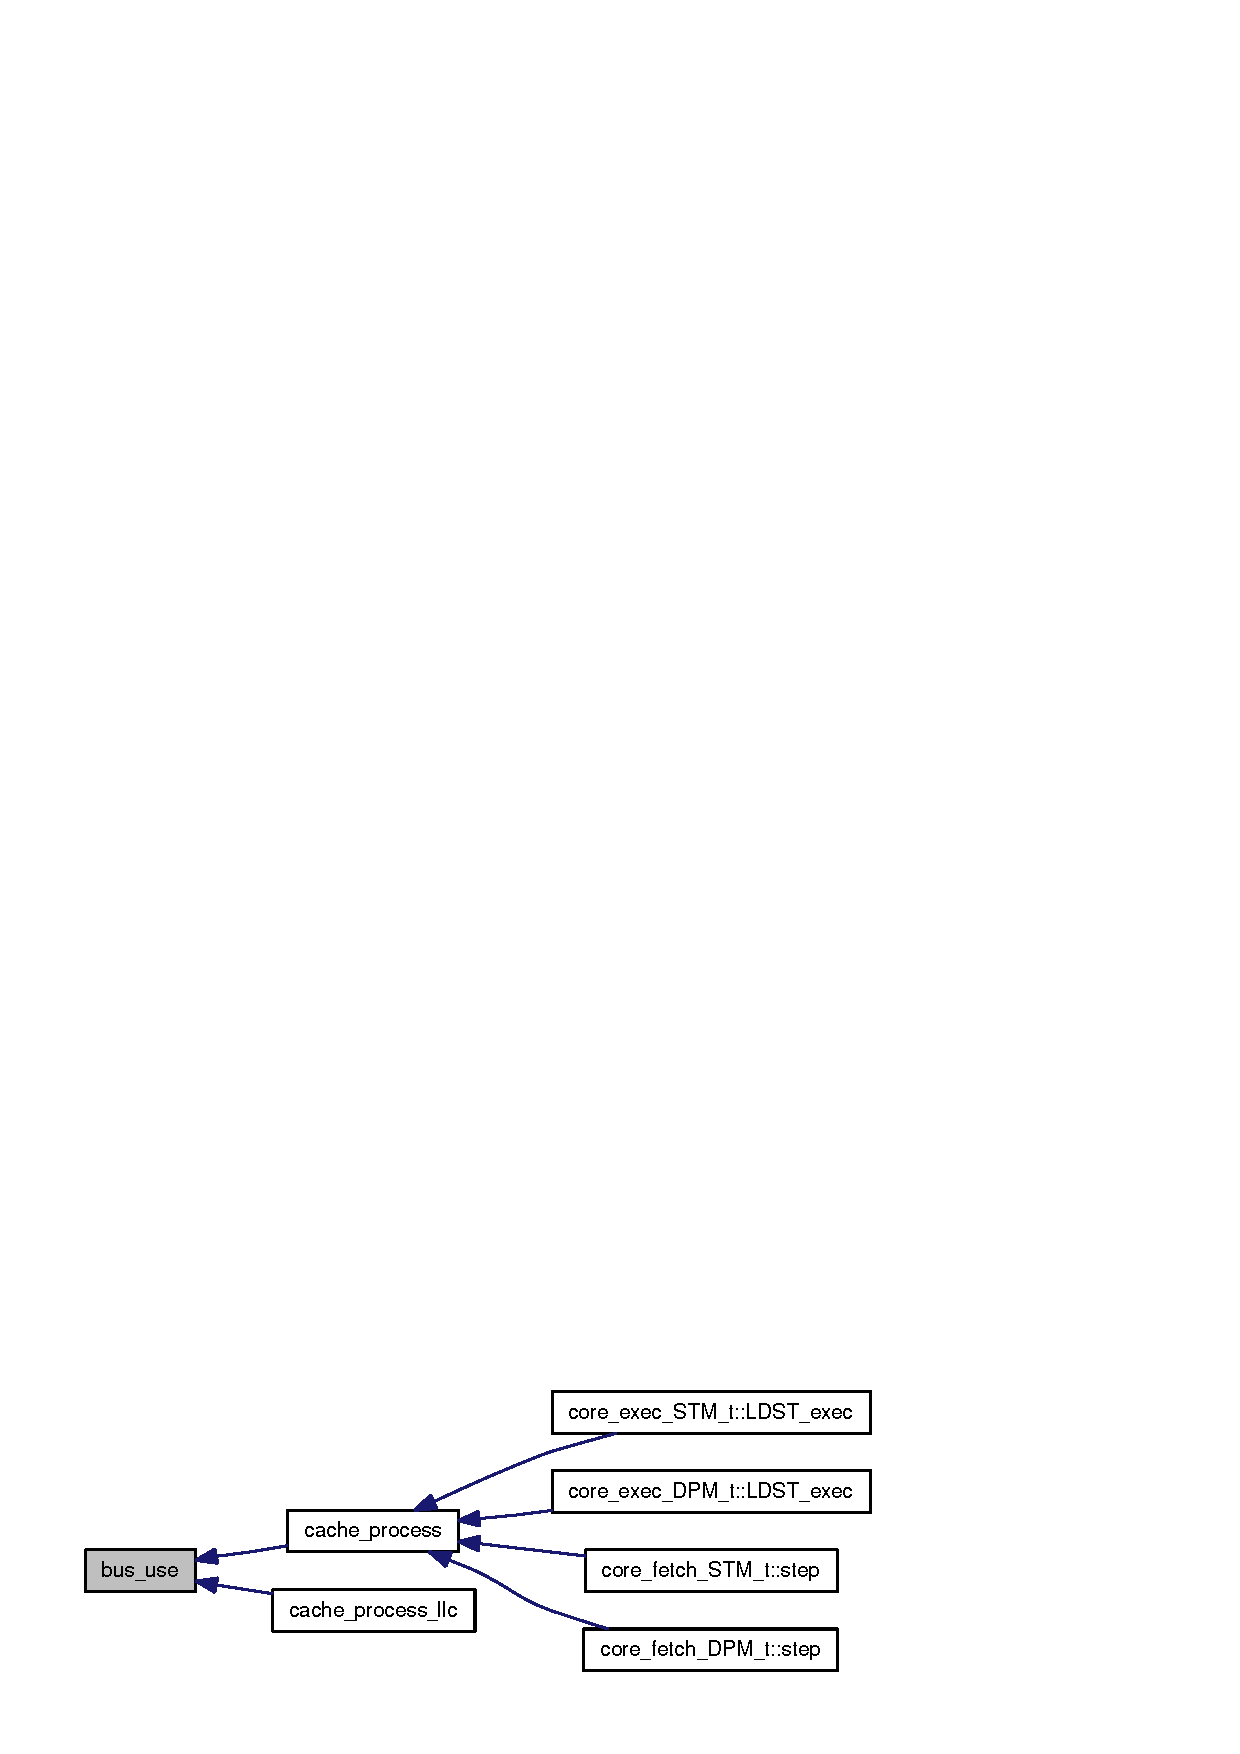
\includegraphics[width=211pt]{zesto-cache_8h_cb6440bff7b9405665cbae0d836630f3_icgraph}
\end{center}
\end{figure}
\index{zesto-cache.h@{zesto-cache.h}!cache\_\-create@{cache\_\-create}}
\index{cache\_\-create@{cache\_\-create}!zesto-cache.h@{zesto-cache.h}}
\subsubsection[{cache\_\-create}]{\setlength{\rightskip}{0pt plus 5cm}struct {\bf cache\_\-t}$\ast$ cache\_\-create (struct {\bf core\_\-t} $\ast$const  {\em core}, \/  const char $\ast$const  {\em name}, \/  const bool {\em read\_\-only}, \/  const int {\em sets}, \/  const int {\em assoc}, \/  const int {\em linesize}, \/  const char {\em rp}, \/  const char {\em ap}, \/  const char {\em wp}, \/  const char {\em wc}, \/  const int {\em banks}, \/  const int {\em bank\_\-width}, \/  const int {\em latency}, \/  const int {\em WBB\_\-size}, \/  const int {\em MSHR\_\-size}, \/  const int {\em MSHR\_\-banked}, \/  struct {\bf cache\_\-t} $\ast$const  {\em next\_\-level\_\-cache}, \/  struct {\bf bus\_\-t} $\ast$const  {\em bus\_\-next})\hspace{0.3cm}{\tt  [read]}}\label{zesto-cache_8h_f37d0719955363306947d707ca6a56f3}




Definition at line 88 of file config/zesto-cache.cpp.

References cache\_\-t::addr\_\-shift, cache\_\-t::allocate\_\-policy, cache\_\-t::assoc, cache\_\-t::bank\_\-mask, cache\_\-t::bank\_\-shift, cache\_\-t::bank\_\-width, cache\_\-t::banks, cache\_\-t::blocks, cache\_\-t::check\_\-for\_\-MSHR\_\-fill\_\-work, cache\_\-t::check\_\-for\_\-work, cache\_\-t::core, cache\_\-t::core\_\-lookups, cache\_\-t::core\_\-misses, fatal(), cache\_\-t::fill\_\-num, cache\_\-t::fill\_\-pipe, cache\_\-t::heap\_\-size, cache\_\-t::latency, cache\_\-t::linesize, cache\_\-t::log2\_\-assoc, cache\_\-t::MSHR, cache\_\-t::MSHR\_\-banks, cache\_\-t::MSHR\_\-mask, cache\_\-t::MSHR\_\-size, mytoupper(), cache\_\-t::name, cache\_\-line\_\-t::next, cache\_\-t::next\_\-bus, cache\_\-t::next\_\-level, NO\_\-WRITE\_\-ALLOC, num\_\-threads, cache\_\-t::pipe, cache\_\-t::pipe\_\-num, cache\_\-t::read\_\-only, REPLACE\_\-CLOCK, REPLACE\_\-LRU, REPLACE\_\-MRU, REPLACE\_\-NMRU, REPLACE\_\-PLRU, REPLACE\_\-RANDOM, cache\_\-t::replacement\_\-policy, cache\_\-t::sets, cache\_\-t::stat, cache\_\-line\_\-t::way, cache\_\-t::WBB, cache\_\-t::WBB\_\-head, cache\_\-t::WBB\_\-num, cache\_\-t::WBB\_\-size, cache\_\-t::WBB\_\-tail, WRITE\_\-ALLOC, WRITE\_\-BACK, cache\_\-t::write\_\-combining, cache\_\-t::write\_\-policy, and WRITE\_\-THROUGH.

Referenced by core\_\-exec\_\-DPM\_\-t::core\_\-exec\_\-DPM\_\-t(), core\_\-exec\_\-STM\_\-t::core\_\-exec\_\-STM\_\-t(), core\_\-fetch\_\-DPM\_\-t::core\_\-fetch\_\-DPM\_\-t(), and core\_\-fetch\_\-STM\_\-t::core\_\-fetch\_\-STM\_\-t().

Here is the caller graph for this function:\nopagebreak
\begin{figure}[H]
\begin{center}
\leavevmode
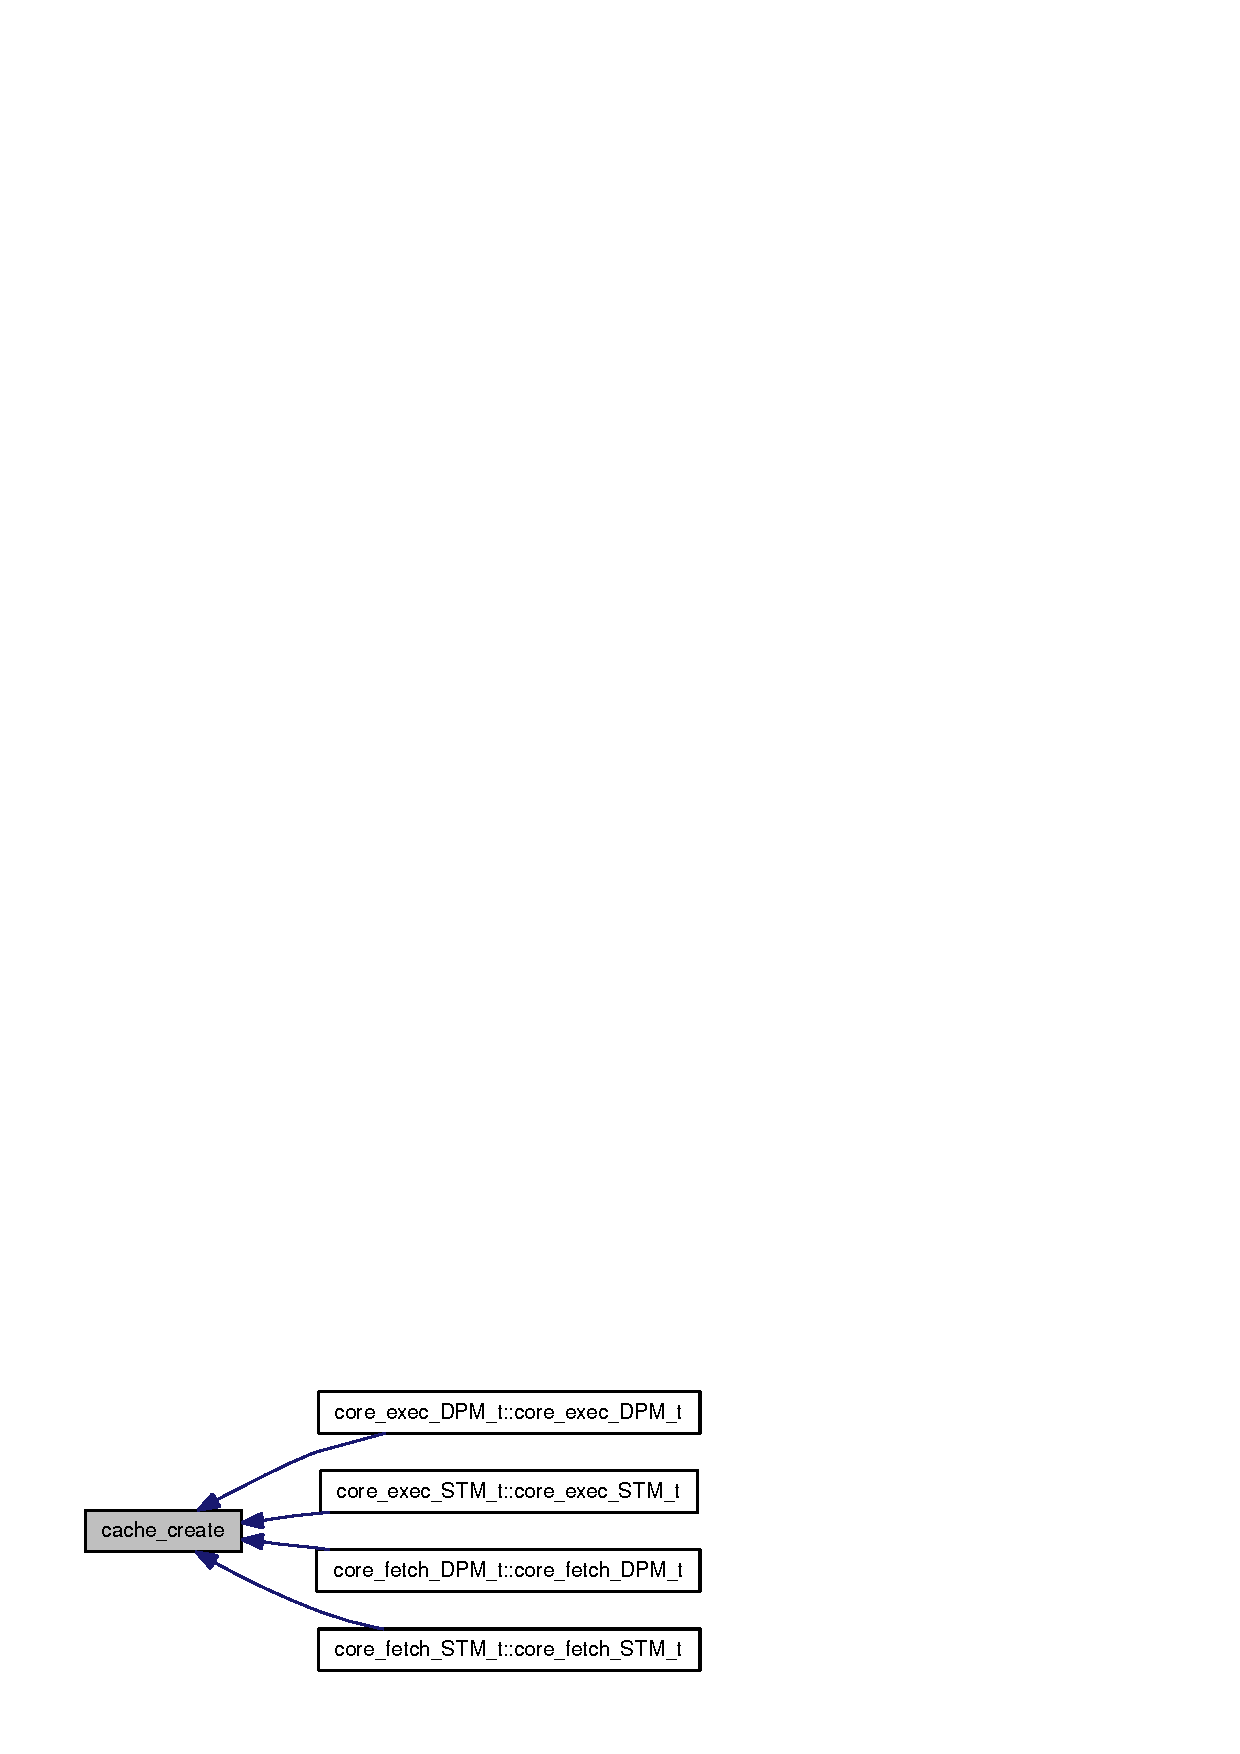
\includegraphics[width=170pt]{zesto-cache_8h_f37d0719955363306947d707ca6a56f3_icgraph}
\end{center}
\end{figure}
\index{zesto-cache.h@{zesto-cache.h}!cache\_\-create\_\-llc@{cache\_\-create\_\-llc}}
\index{cache\_\-create\_\-llc@{cache\_\-create\_\-llc}!zesto-cache.h@{zesto-cache.h}}
\subsubsection[{cache\_\-create\_\-llc}]{\setlength{\rightskip}{0pt plus 5cm}struct {\bf cache\_\-t}$\ast$ cache\_\-create\_\-llc (struct {\bf core\_\-t} $\ast$const  {\em core}, \/  const char $\ast$const  {\em name}, \/  const bool {\em read\_\-only}, \/  const int {\em sets}, \/  const int {\em assoc}, \/  const int {\em linesize}, \/  const char {\em rp}, \/  const char {\em ap}, \/  const char {\em wp}, \/  const char {\em wc}, \/  const int {\em banks}, \/  const int {\em bank\_\-width}, \/  const int {\em latency}, \/  const int {\em WBB\_\-size}, \/  const int {\em MSHR\_\-size}, \/  const int {\em MSHR\_\-banked}, \/  const int {\em begin\_\-index}, \/  const int {\em end\_\-index}, \/  struct {\bf cache\_\-t} $\ast$const  {\em next\_\-level\_\-cache}, \/  struct {\bf bus\_\-t} $\ast$const  {\em bus\_\-next})\hspace{0.3cm}{\tt  [read]}}\label{zesto-cache_8h_8e1bb5340056d589c19813cbc1ab6318}




Definition at line 87 of file config/zesto-llc.cpp.

References cache\_\-t::addr\_\-shift, cache\_\-t::allocate\_\-policy, cache\_\-t::assoc, cache\_\-t::bank\_\-mask, cache\_\-t::bank\_\-shift, cache\_\-t::bank\_\-width, cache\_\-t::banks, cache\_\-t::blocks, cache\_\-t::check\_\-for\_\-MSHR\_\-fill\_\-work, cache\_\-t::check\_\-for\_\-work, cache\_\-t::core, cache\_\-t::core\_\-lookups, cache\_\-t::core\_\-misses, fatal(), cache\_\-t::fill\_\-num, cache\_\-t::fill\_\-pipe, cache\_\-t::heap\_\-size, cache\_\-t::latency, cache\_\-t::linesize, cache\_\-t::log2\_\-assoc, cache\_\-t::MSHR, cache\_\-t::MSHR\_\-banks, cache\_\-t::MSHR\_\-mask, cache\_\-t::MSHR\_\-size, mytoupper(), cache\_\-t::name, cache\_\-line\_\-t::next, cache\_\-t::next\_\-bus, cache\_\-t::next\_\-level, NO\_\-WRITE\_\-ALLOC, num\_\-threads, cache\_\-t::pipe, cache\_\-t::pipe\_\-num, cache\_\-t::read\_\-only, REPLACE\_\-CLOCK, REPLACE\_\-LRU, REPLACE\_\-MRU, REPLACE\_\-NMRU, REPLACE\_\-PLRU, REPLACE\_\-RANDOM, cache\_\-t::replacement\_\-policy, cache\_\-t::sets, cache\_\-t::stat, cache\_\-line\_\-t::way, cache\_\-t::WBB, cache\_\-t::WBB\_\-head, cache\_\-t::WBB\_\-num, cache\_\-t::WBB\_\-size, cache\_\-t::WBB\_\-tail, WRITE\_\-ALLOC, WRITE\_\-BACK, cache\_\-t::write\_\-combining, cache\_\-t::write\_\-policy, and WRITE\_\-THROUGH.\index{zesto-cache.h@{zesto-cache.h}!cache\_\-enqueuable@{cache\_\-enqueuable}}
\index{cache\_\-enqueuable@{cache\_\-enqueuable}!zesto-cache.h@{zesto-cache.h}}
\subsubsection[{cache\_\-enqueuable}]{\setlength{\rightskip}{0pt plus 5cm}int cache\_\-enqueuable (const struct {\bf cache\_\-t} $\ast$const  {\em cp}, \/  const int {\em thread\_\-id}, \/  const {\bf md\_\-paddr\_\-t} {\em addr})}\label{zesto-cache_8h_35c7c82c117f5713ec55d40f831060da}




Definition at line 1076 of file config/zesto-cache.cpp.

References DO\_\-NOT\_\-TRANSLATE, GET\_\-BANK, cache\_\-t::latency, and cache\_\-t::pipe\_\-num.

Referenced by cache\_\-prefetch(), cache\_\-prefetch\_\-llc(), cache\_\-process(), core\_\-exec\_\-STM\_\-t::LDQ\_\-schedule(), core\_\-exec\_\-DPM\_\-t::LDQ\_\-schedule(), core\_\-fetch\_\-STM\_\-t::step(), core\_\-fetch\_\-DPM\_\-t::step(), core\_\-exec\_\-STM\_\-t::STQ\_\-deallocate\_\-std(), and core\_\-exec\_\-DPM\_\-t::STQ\_\-deallocate\_\-std().

Here is the caller graph for this function:\nopagebreak
\begin{figure}[H]
\begin{center}
\leavevmode
\includegraphics[width=420pt]{zesto-cache_8h_35c7c82c117f5713ec55d40f831060da_icgraph}
\end{center}
\end{figure}
\index{zesto-cache.h@{zesto-cache.h}!cache\_\-enqueuable\_\-llc@{cache\_\-enqueuable\_\-llc}}
\index{cache\_\-enqueuable\_\-llc@{cache\_\-enqueuable\_\-llc}!zesto-cache.h@{zesto-cache.h}}
\subsubsection[{cache\_\-enqueuable\_\-llc}]{\setlength{\rightskip}{0pt plus 5cm}int cache\_\-enqueuable\_\-llc (const struct {\bf cache\_\-t} $\ast$const  {\em cp}, \/  const int {\em thread\_\-id}, \/  const {\bf md\_\-paddr\_\-t} {\em addr})}\label{zesto-cache_8h_17919e2800a0393570b40f08156cb42c}




Definition at line 989 of file config/zesto-llc.cpp.

References DO\_\-NOT\_\-TRANSLATE, GET\_\-BANK, cache\_\-t::latency, and cache\_\-t::pipe\_\-num.\index{zesto-cache.h@{zesto-cache.h}!cache\_\-enqueue@{cache\_\-enqueue}}
\index{cache\_\-enqueue@{cache\_\-enqueue}!zesto-cache.h@{zesto-cache.h}}
\subsubsection[{cache\_\-enqueue}]{\setlength{\rightskip}{0pt plus 5cm}void cache\_\-enqueue (struct {\bf core\_\-t} $\ast$const  {\em core}, \/  struct {\bf cache\_\-t} $\ast$const  {\em cp}, \/  struct {\bf cache\_\-t} $\ast$const  {\em prev\_\-cp}, \/  const enum {\bf cache\_\-command} {\em cmd}, \/  const int {\em thread\_\-id}, \/  const {\bf md\_\-addr\_\-t} {\em PC}, \/  const {\bf md\_\-paddr\_\-t} {\em addr}, \/  const {\bf seq\_\-t} {\em action\_\-id}, \/  const int {\em MSHR\_\-bank}, \/  const int {\em MSHR\_\-index}, \/  void $\ast$const  {\em op}, \/  void($\ast$)(void $\ast$) {\em cb}, \/  void($\ast$)(void $\ast$, int) {\em miss\_\-cb}, \/  bool($\ast$)(void $\ast$, {\bf seq\_\-t}) {\em translated\_\-cb}, \/  {\bf seq\_\-t}($\ast$)(void $\ast$) {\em get\_\-action\_\-id})}\label{zesto-cache_8h_0831369c0f015a2e350b71f2fc445c70}




Definition at line 1095 of file config/zesto-cache.cpp.

References cache\_\-action\_\-t::action\_\-id, cache\_\-assert, cache\_\-heap\_\-balance(), cache\_\-action\_\-t::cb, cache\_\-t::check\_\-for\_\-pipe\_\-work, cache\_\-t::check\_\-for\_\-work, cache\_\-action\_\-t::cmd, cache\_\-action\_\-t::core, DO\_\-NOT\_\-TRANSLATE, cache\_\-action\_\-t::get\_\-action\_\-id, GET\_\-BANK, cache\_\-t::latency, cache\_\-action\_\-t::miss\_\-cb, cache\_\-action\_\-t::miss\_\-cb\_\-invoked, cache\_\-action\_\-t::MSHR\_\-bank, cache\_\-action\_\-t::MSHR\_\-index, cache\_\-action\_\-t::op, cache\_\-action\_\-t::paddr, cache\_\-action\_\-t::PC, cache\_\-t::pipe, cache\_\-action\_\-t::pipe\_\-exit\_\-time, cache\_\-t::pipe\_\-num, cache\_\-action\_\-t::prev\_\-cp, sim\_\-cycle, TICK\_\-T\_\-MAX, cache\_\-action\_\-t::translated\_\-cb, cache\_\-action\_\-t::when\_\-returned, and cache\_\-action\_\-t::when\_\-started.

Referenced by cache\_\-prefetch(), cache\_\-prefetch\_\-llc(), cache\_\-process(), core\_\-exec\_\-STM\_\-t::LDQ\_\-schedule(), core\_\-exec\_\-DPM\_\-t::LDQ\_\-schedule(), core\_\-fetch\_\-STM\_\-t::step(), core\_\-fetch\_\-DPM\_\-t::step(), core\_\-exec\_\-STM\_\-t::STQ\_\-deallocate\_\-std(), and core\_\-exec\_\-DPM\_\-t::STQ\_\-deallocate\_\-std().

Here is the caller graph for this function:\nopagebreak
\begin{figure}[H]
\begin{center}
\leavevmode
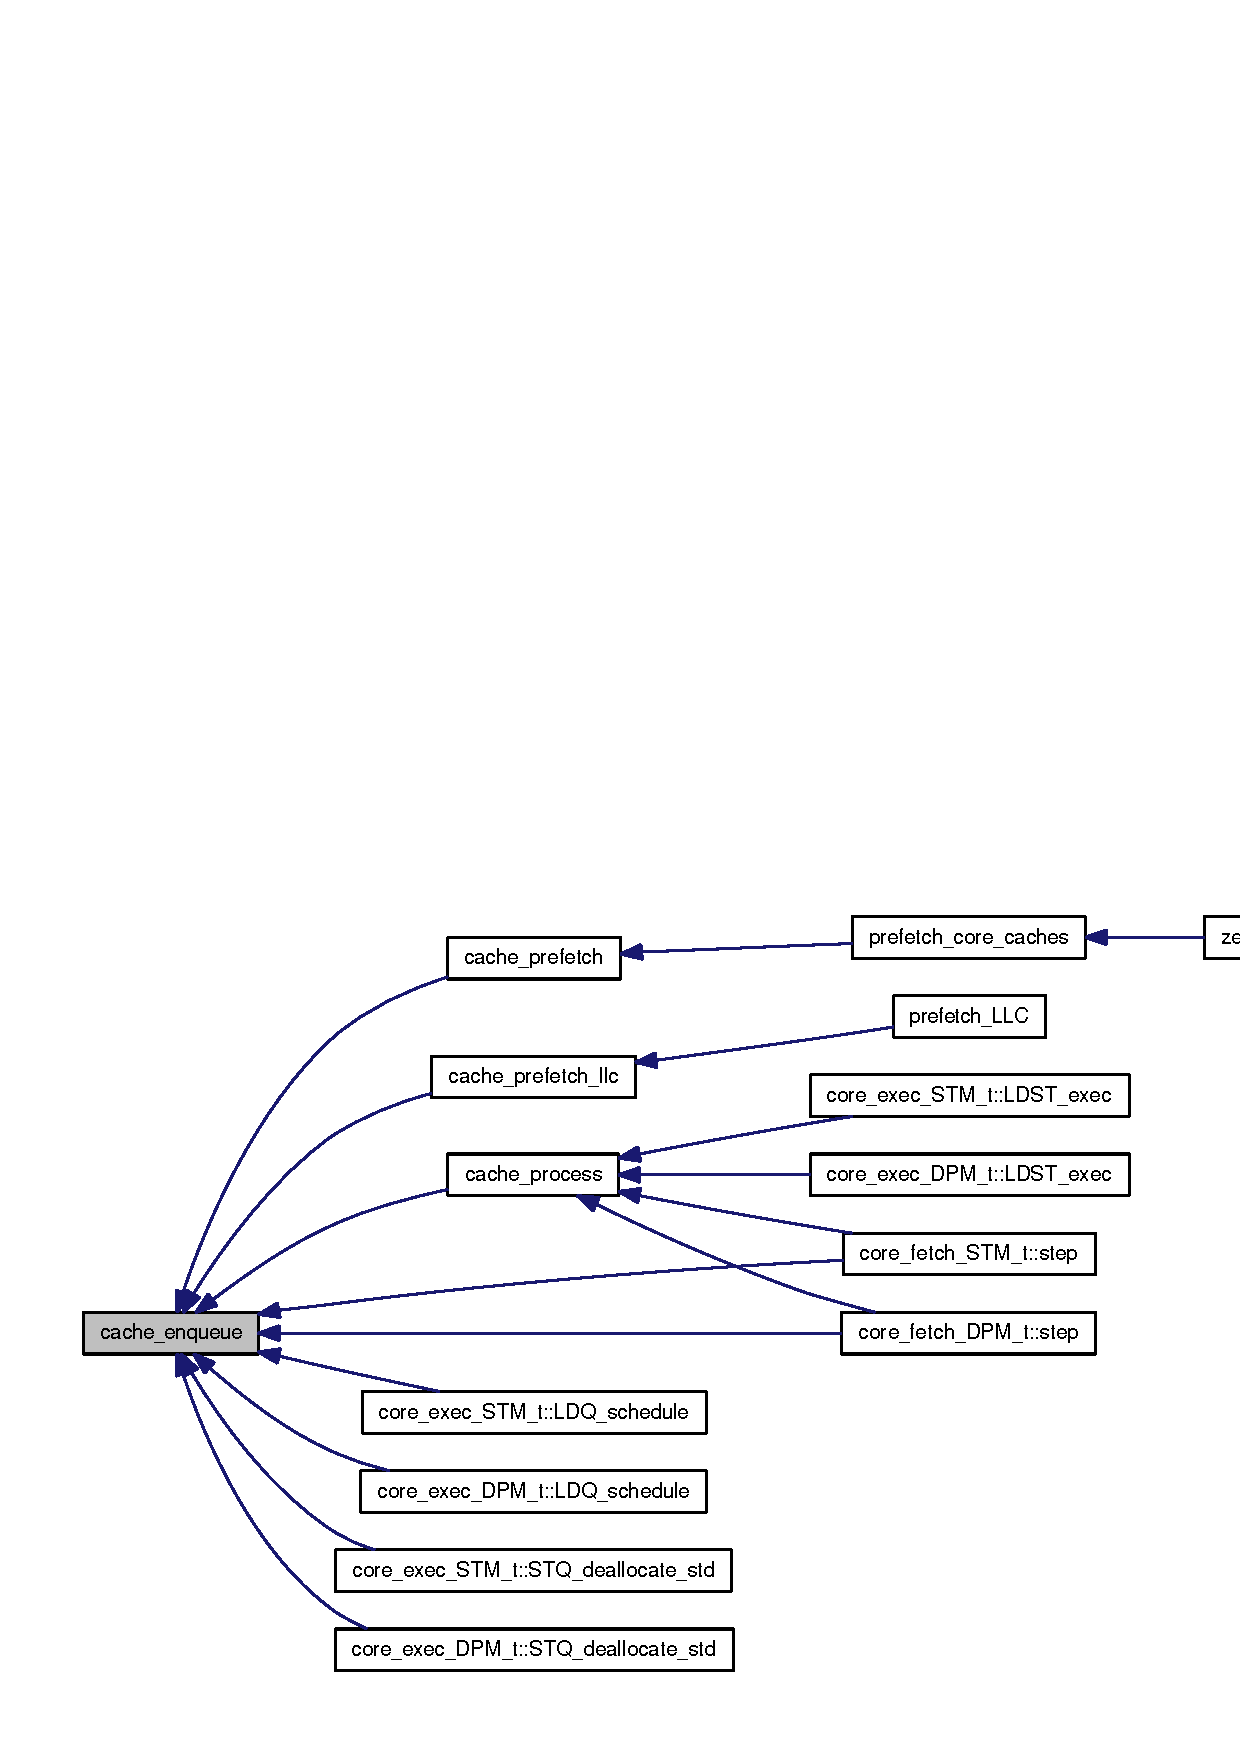
\includegraphics[width=420pt]{zesto-cache_8h_0831369c0f015a2e350b71f2fc445c70_icgraph}
\end{center}
\end{figure}
\index{zesto-cache.h@{zesto-cache.h}!cache\_\-enqueue\_\-llc@{cache\_\-enqueue\_\-llc}}
\index{cache\_\-enqueue\_\-llc@{cache\_\-enqueue\_\-llc}!zesto-cache.h@{zesto-cache.h}}
\subsubsection[{cache\_\-enqueue\_\-llc}]{\setlength{\rightskip}{0pt plus 5cm}void cache\_\-enqueue\_\-llc (struct {\bf core\_\-t} $\ast$const  {\em core}, \/  struct {\bf cache\_\-t} $\ast$const  {\em cp}, \/  struct {\bf cache\_\-t} $\ast$const  {\em prev\_\-cp}, \/  const enum {\bf cache\_\-command} {\em cmd}, \/  const int {\em thread\_\-id}, \/  const {\bf md\_\-addr\_\-t} {\em PC}, \/  const {\bf md\_\-paddr\_\-t} {\em addr}, \/  const {\bf seq\_\-t} {\em action\_\-id}, \/  const int {\em MSHR\_\-bank}, \/  const int {\em MSHR\_\-index}, \/  void $\ast$const  {\em op}, \/  void($\ast$)(void $\ast$) {\em cb}, \/  void($\ast$)(void $\ast$, int) {\em miss\_\-cb}, \/  bool($\ast$)(void $\ast$, {\bf seq\_\-t}) {\em translated\_\-cb}, \/  {\bf seq\_\-t}($\ast$)(void $\ast$) {\em get\_\-action\_\-id})}\label{zesto-cache_8h_6955e78ccb0fb1511754e8cd113e1dcc}




Definition at line 1008 of file config/zesto-llc.cpp.

References cache\_\-action\_\-t::action\_\-id, cache\_\-assert, cache\_\-heap\_\-balance(), cache\_\-action\_\-t::cb, cache\_\-t::check\_\-for\_\-pipe\_\-work, cache\_\-t::check\_\-for\_\-work, cache\_\-action\_\-t::cmd, cache\_\-action\_\-t::core, DO\_\-NOT\_\-TRANSLATE, cache\_\-action\_\-t::get\_\-action\_\-id, GET\_\-BANK, cache\_\-t::latency, cache\_\-action\_\-t::miss\_\-cb, cache\_\-action\_\-t::miss\_\-cb\_\-invoked, cache\_\-action\_\-t::MSHR\_\-bank, cache\_\-action\_\-t::MSHR\_\-index, cache\_\-action\_\-t::op, cache\_\-action\_\-t::paddr, cache\_\-action\_\-t::PC, cache\_\-t::pipe, cache\_\-action\_\-t::pipe\_\-exit\_\-time, cache\_\-t::pipe\_\-num, cache\_\-action\_\-t::prev\_\-cp, sim\_\-cycle, TICK\_\-T\_\-MAX, cache\_\-action\_\-t::translated\_\-cb, cache\_\-action\_\-t::when\_\-returned, and cache\_\-action\_\-t::when\_\-started.\index{zesto-cache.h@{zesto-cache.h}!cache\_\-freeze\_\-stats@{cache\_\-freeze\_\-stats}}
\index{cache\_\-freeze\_\-stats@{cache\_\-freeze\_\-stats}!zesto-cache.h@{zesto-cache.h}}
\subsubsection[{cache\_\-freeze\_\-stats}]{\setlength{\rightskip}{0pt plus 5cm}void cache\_\-freeze\_\-stats (struct {\bf core\_\-t} $\ast$const  {\em core})}\label{zesto-cache_8h_bd1fe8334f2259dc773b85f98c7fbcfa}




Definition at line 2402 of file config/zesto-cache.cpp.

References core\_\-t::core\_\-t::core\_\-memory\_\-t::DL1, core\_\-t::core\_\-t::core\_\-memory\_\-t::DL2, core\_\-t::core\_\-t::core\_\-memory\_\-t::DTLB, core\_\-t::core\_\-t::core\_\-memory\_\-t::DTLB2, cache\_\-t::frozen, core\_\-t::core\_\-t::core\_\-memory\_\-t::IL1, core\_\-t::core\_\-t::core\_\-memory\_\-t::ITLB, and core\_\-t::memory.

Referenced by core\_\-commit\_\-STM\_\-t::step(), and core\_\-commit\_\-DPM\_\-t::step().

Here is the caller graph for this function:\nopagebreak
\begin{figure}[H]
\begin{center}
\leavevmode
\includegraphics[width=157pt]{zesto-cache_8h_bd1fe8334f2259dc773b85f98c7fbcfa_icgraph}
\end{center}
\end{figure}
\index{zesto-cache.h@{zesto-cache.h}!cache\_\-get\_\-evictee@{cache\_\-get\_\-evictee}}
\index{cache\_\-get\_\-evictee@{cache\_\-get\_\-evictee}!zesto-cache.h@{zesto-cache.h}}
\subsubsection[{cache\_\-get\_\-evictee}]{\setlength{\rightskip}{0pt plus 5cm}struct {\bf cache\_\-line\_\-t}$\ast$ cache\_\-get\_\-evictee (struct {\bf cache\_\-t} $\ast$const  {\em cp}, \/  const {\bf md\_\-paddr\_\-t} {\em addr}, \/  struct {\bf core\_\-t} $\ast$const  {\em core})\hspace{0.3cm}{\tt  [read]}}\label{zesto-cache_8h_ff8ad962ac5134671915f22e604a2f4e}




Definition at line 840 of file config/zesto-cache.cpp.

References cache\_\-t::addr\_\-shift, cache\_\-t::assoc, cache\_\-t::blocks, fatal(), cache\_\-t::log2\_\-assoc, cache\_\-line\_\-t::meta, modinc(), cache\_\-t::name, cache\_\-line\_\-t::next, REPLACE\_\-CLOCK, REPLACE\_\-LRU, REPLACE\_\-MRU, REPLACE\_\-NMRU, REPLACE\_\-PLRU, REPLACE\_\-RANDOM, cache\_\-t::replacement\_\-policy, cache\_\-t::sets, cache\_\-line\_\-t::valid, and cache\_\-line\_\-t::way.

Referenced by cache\_\-process(), and sim\_\-fastfwd().

Here is the caller graph for this function:\nopagebreak
\begin{figure}[H]
\begin{center}
\leavevmode
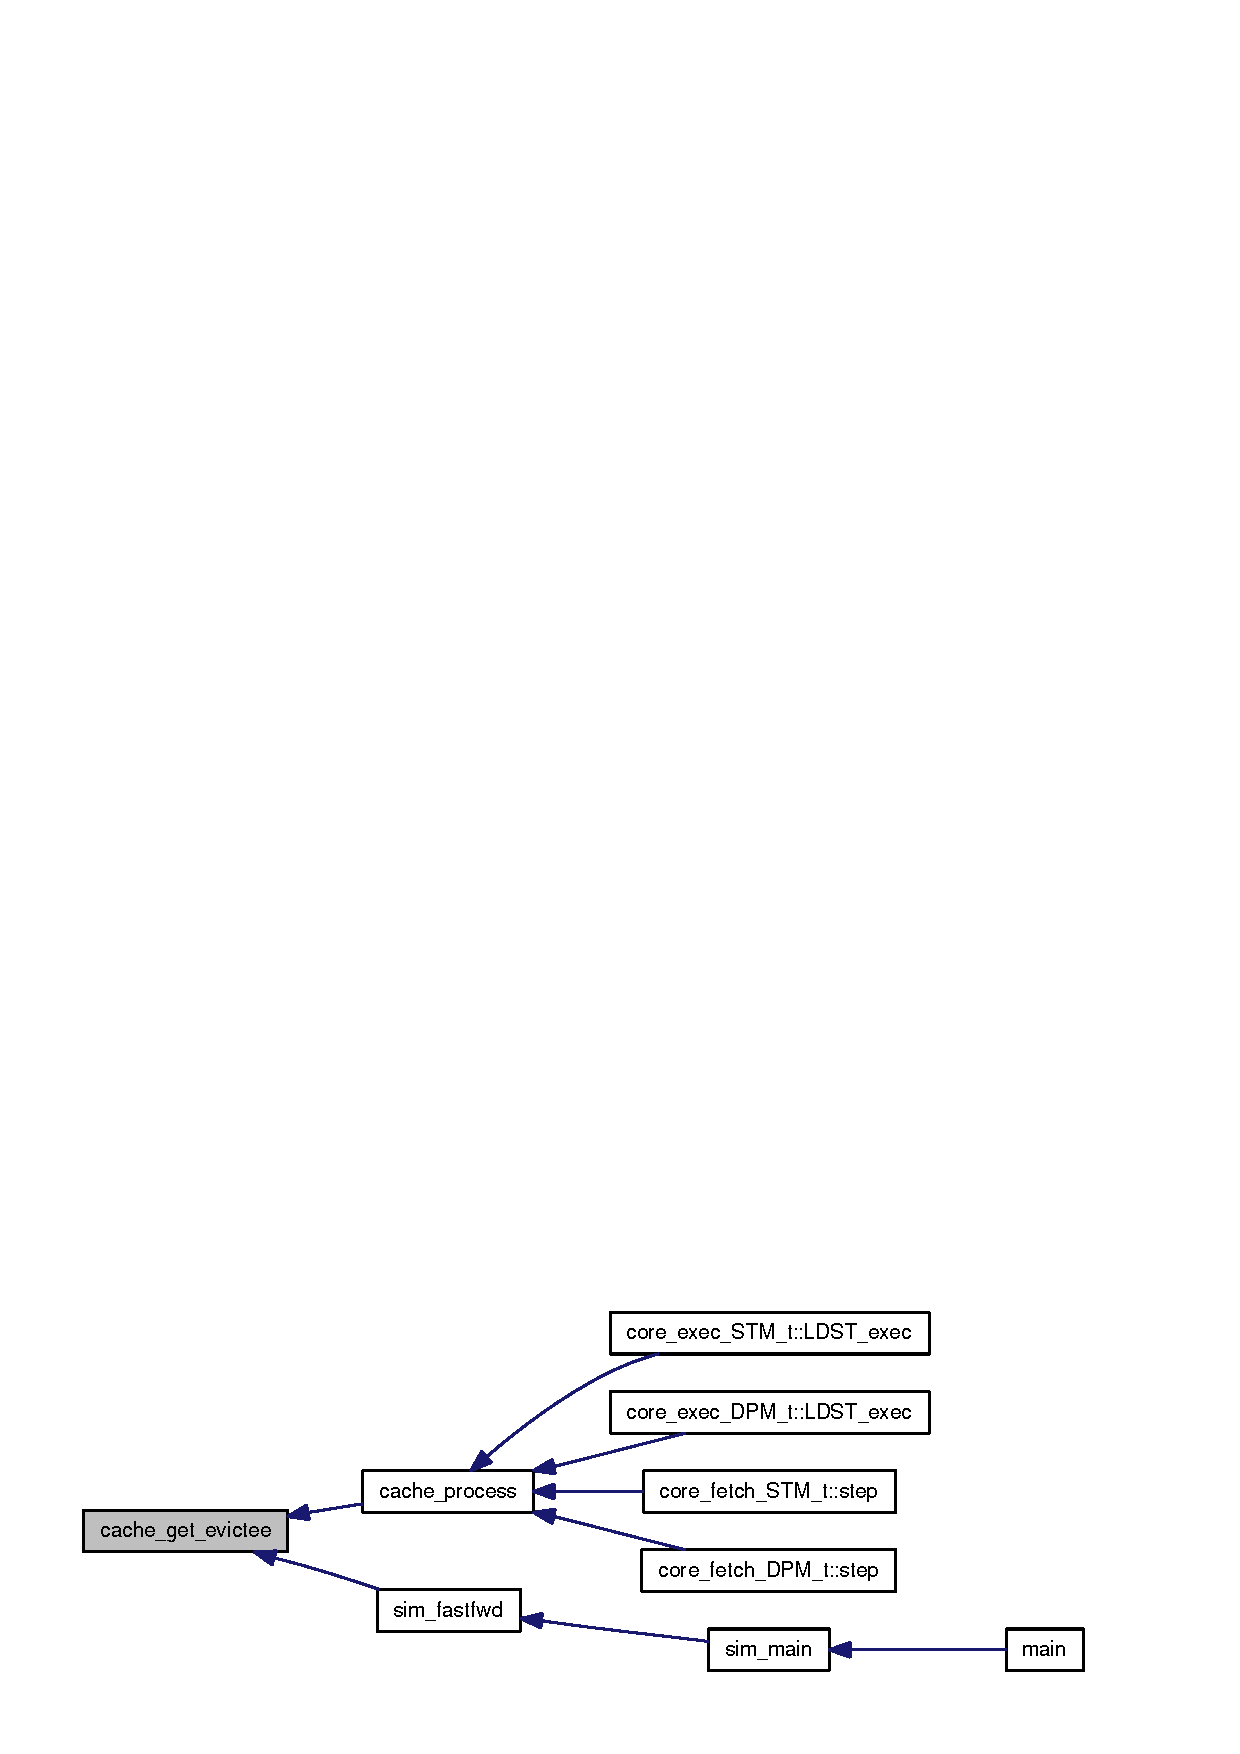
\includegraphics[width=262pt]{zesto-cache_8h_ff8ad962ac5134671915f22e604a2f4e_icgraph}
\end{center}
\end{figure}
\index{zesto-cache.h@{zesto-cache.h}!cache\_\-get\_\-evictee\_\-llc@{cache\_\-get\_\-evictee\_\-llc}}
\index{cache\_\-get\_\-evictee\_\-llc@{cache\_\-get\_\-evictee\_\-llc}!zesto-cache.h@{zesto-cache.h}}
\subsubsection[{cache\_\-get\_\-evictee\_\-llc}]{\setlength{\rightskip}{0pt plus 5cm}struct {\bf cache\_\-line\_\-t}$\ast$ cache\_\-get\_\-evictee\_\-llc (struct {\bf cache\_\-t} $\ast$const  {\em cp}, \/  const {\bf md\_\-paddr\_\-t} {\em addr}, \/  struct {\bf core\_\-t} $\ast$const  {\em core})\hspace{0.3cm}{\tt  [read]}}\label{zesto-cache_8h_77864b4219a45ec15cbe3ff986d131b9}




Definition at line 751 of file config/zesto-llc.cpp.

References cache\_\-t::addr\_\-shift, cache\_\-t::assoc, cache\_\-t::blocks, fatal(), cache\_\-t::log2\_\-assoc, cache\_\-line\_\-t::meta, modinc(), cache\_\-t::name, cache\_\-line\_\-t::next, REPLACE\_\-CLOCK, REPLACE\_\-LRU, REPLACE\_\-MRU, REPLACE\_\-NMRU, REPLACE\_\-PLRU, REPLACE\_\-RANDOM, cache\_\-t::replacement\_\-policy, cache\_\-t::sets, cache\_\-line\_\-t::valid, and cache\_\-line\_\-t::way.\index{zesto-cache.h@{zesto-cache.h}!cache\_\-insert\_\-block@{cache\_\-insert\_\-block}}
\index{cache\_\-insert\_\-block@{cache\_\-insert\_\-block}!zesto-cache.h@{zesto-cache.h}}
\subsubsection[{cache\_\-insert\_\-block}]{\setlength{\rightskip}{0pt plus 5cm}void cache\_\-insert\_\-block (struct {\bf cache\_\-t} $\ast$const  {\em cp}, \/  const enum {\bf cache\_\-command} {\em cmd}, \/  const {\bf md\_\-paddr\_\-t} {\em addr}, \/  struct {\bf core\_\-t} $\ast$const  {\em core})}\label{zesto-cache_8h_219ea5df10c94dbf2c820586f981158f}




Definition at line 742 of file config/zesto-cache.cpp.

References cache\_\-t::addr\_\-shift, cache\_\-t::blocks, cache\_\-assert, CACHE\_\-PREFETCH, CACHE\_\-STAT, CACHE\_\-WRITE, CACHE\_\-WRITEBACK, cache\_\-line\_\-t::core, cache\_\-line\_\-t::dirty, fatal(), cache\_\-t::log2\_\-assoc, cache\_\-line\_\-t::meta, cache\_\-line\_\-t::next, cache\_\-t::prefetch\_\-insertions, cache\_\-line\_\-t::prefetched, REPLACE\_\-CLOCK, REPLACE\_\-LRU, REPLACE\_\-MRU, REPLACE\_\-NMRU, REPLACE\_\-PLRU, REPLACE\_\-RANDOM, cache\_\-t::replacement\_\-policy, cache\_\-t::sets, cache\_\-t::stat, cache\_\-line\_\-t::tag, cache\_\-line\_\-t::valid, and cache\_\-line\_\-t::way.

Referenced by cache\_\-process(), and sim\_\-fastfwd().

Here is the caller graph for this function:\nopagebreak
\begin{figure}[H]
\begin{center}
\leavevmode
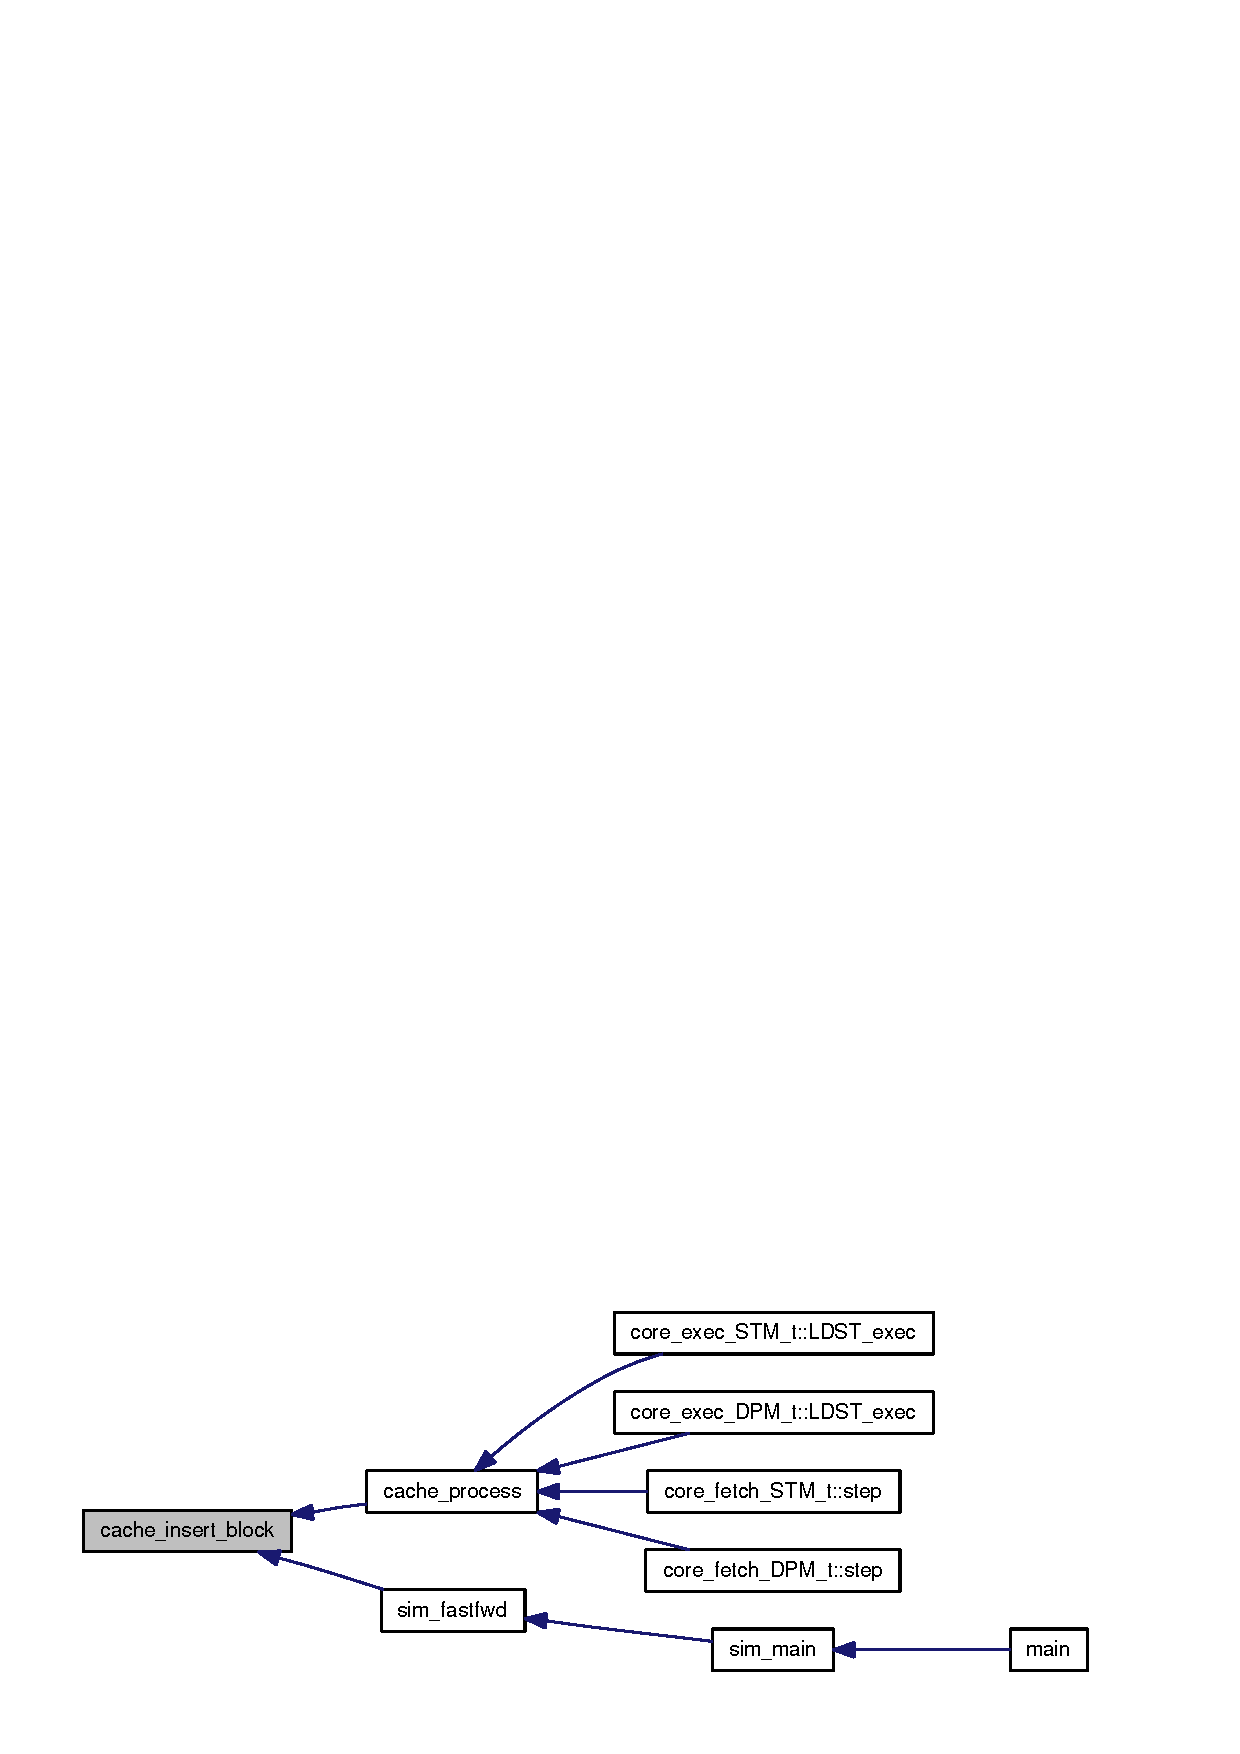
\includegraphics[width=263pt]{zesto-cache_8h_219ea5df10c94dbf2c820586f981158f_icgraph}
\end{center}
\end{figure}
\index{zesto-cache.h@{zesto-cache.h}!cache\_\-insert\_\-block\_\-llc@{cache\_\-insert\_\-block\_\-llc}}
\index{cache\_\-insert\_\-block\_\-llc@{cache\_\-insert\_\-block\_\-llc}!zesto-cache.h@{zesto-cache.h}}
\subsubsection[{cache\_\-insert\_\-block\_\-llc}]{\setlength{\rightskip}{0pt plus 5cm}void cache\_\-insert\_\-block\_\-llc (struct {\bf cache\_\-t} $\ast$const  {\em cp}, \/  const enum {\bf cache\_\-command} {\em cmd}, \/  const {\bf md\_\-paddr\_\-t} {\em addr}, \/  struct {\bf core\_\-t} $\ast$const  {\em core})}\label{zesto-cache_8h_abc5a15d6fe00d533a2b4b8e4b13cc59}




Definition at line 653 of file config/zesto-llc.cpp.

References cache\_\-t::addr\_\-shift, cache\_\-t::blocks, cache\_\-assert, CACHE\_\-PREFETCH, CACHE\_\-STAT, CACHE\_\-WRITE, CACHE\_\-WRITEBACK, cache\_\-line\_\-t::core, cache\_\-line\_\-t::dirty, fatal(), cache\_\-t::log2\_\-assoc, cache\_\-line\_\-t::meta, cache\_\-line\_\-t::next, cache\_\-t::prefetch\_\-insertions, cache\_\-line\_\-t::prefetched, REPLACE\_\-CLOCK, REPLACE\_\-LRU, REPLACE\_\-MRU, REPLACE\_\-NMRU, REPLACE\_\-PLRU, REPLACE\_\-RANDOM, cache\_\-t::replacement\_\-policy, cache\_\-t::sets, cache\_\-t::stat, cache\_\-line\_\-t::tag, cache\_\-line\_\-t::valid, and cache\_\-line\_\-t::way.\index{zesto-cache.h@{zesto-cache.h}!cache\_\-invalidate@{cache\_\-invalidate}}
\index{cache\_\-invalidate@{cache\_\-invalidate}!zesto-cache.h@{zesto-cache.h}}
\subsubsection[{cache\_\-invalidate}]{\setlength{\rightskip}{0pt plus 5cm}struct {\bf cache\_\-line\_\-t}$\ast$ cache\_\-invalidate (struct {\bf cache\_\-t} $\ast$const  {\em cp}, \/  const {\bf md\_\-paddr\_\-t} {\em addr}, \/  {\bf core\_\-t} $\ast$const  {\em core})\hspace{0.3cm}{\tt  [read]}}\label{zesto-cache_8h_3b38a26dd8bf1670d4bf3055d66cfc8d}




Definition at line 841 of file zesto-cache.cpp.

References cache\_\-t::addr\_\-shift, cache\_\-t::blocks, cache\_\-invalidate(), cache\_\-peek(), cache\_\-line\_\-t::dirty, fatal(), cache\_\-line\_\-t::next, cache\_\-t::prev\_\-level, cache\_\-t::sets, cache\_\-line\_\-t::tag, and cache\_\-line\_\-t::valid.

Referenced by cache\_\-invalidate(), cache\_\-process(), and cache\_\-process\_\-llc().

Here is the caller graph for this function:\nopagebreak
\begin{figure}[H]
\begin{center}
\leavevmode
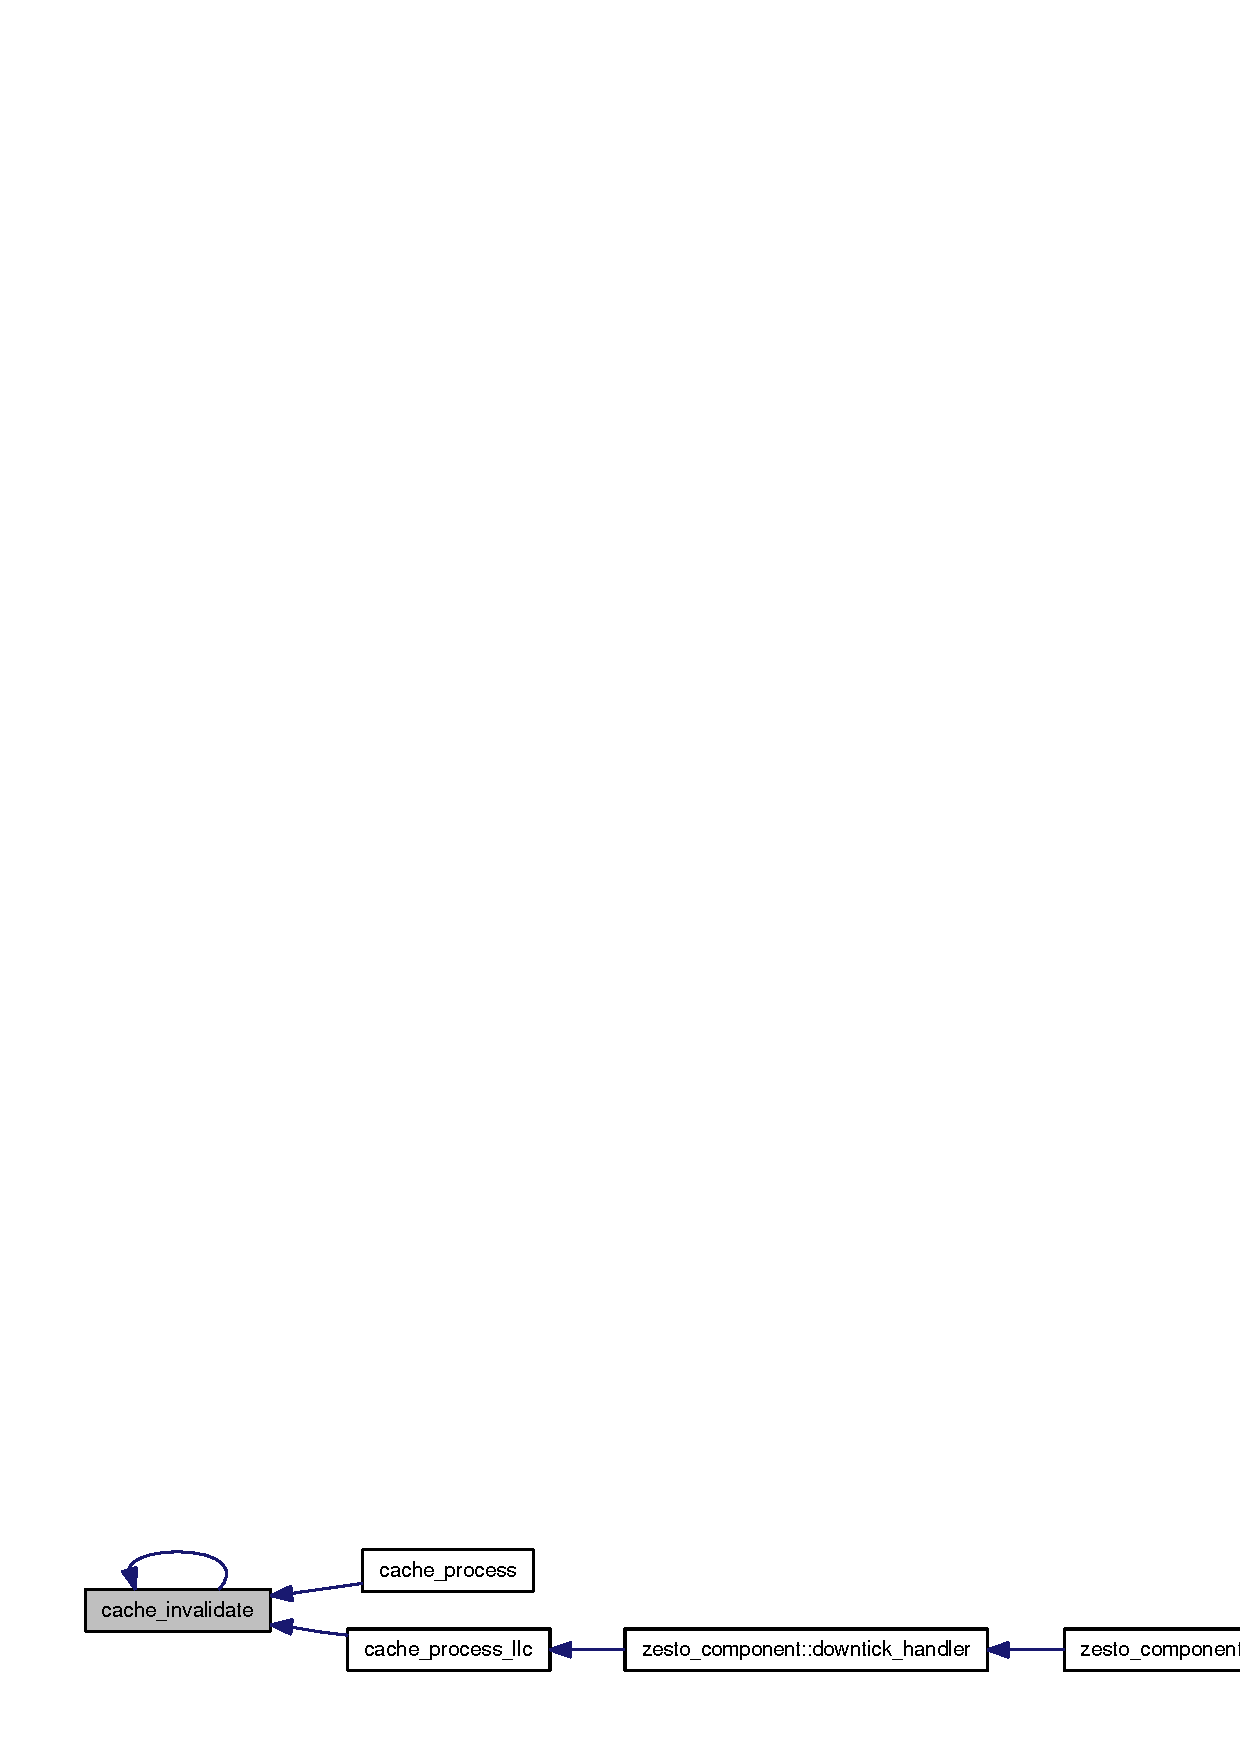
\includegraphics[width=383pt]{zesto-cache_8h_3b38a26dd8bf1670d4bf3055d66cfc8d_icgraph}
\end{center}
\end{figure}
\index{zesto-cache.h@{zesto-cache.h}!cache\_\-is\_\-hit@{cache\_\-is\_\-hit}}
\index{cache\_\-is\_\-hit@{cache\_\-is\_\-hit}!zesto-cache.h@{zesto-cache.h}}
\subsubsection[{cache\_\-is\_\-hit}]{\setlength{\rightskip}{0pt plus 5cm}struct {\bf cache\_\-line\_\-t}$\ast$ cache\_\-is\_\-hit (struct {\bf cache\_\-t} $\ast$const  {\em cp}, \/  const enum {\bf cache\_\-command} {\em cmd}, \/  const {\bf md\_\-paddr\_\-t} {\em addr}, \/  struct {\bf core\_\-t} $\ast$const  {\em core})\hspace{0.3cm}{\tt  [read]}}\label{zesto-cache_8h_bbba2e5ba6186173122bcf1e35dc56eb}




Definition at line 618 of file config/zesto-cache.cpp.

References cache\_\-t::addr\_\-shift, cache\_\-t::blocks, cache\_\-assert, CACHE\_\-READONLY, CACHE\_\-WRITE, CACHE\_\-WRITEBACK, cache\_\-line\_\-t::dirty, fatal(), cache\_\-t::log2\_\-assoc, cache\_\-line\_\-t::meta, cache\_\-line\_\-t::next, cache\_\-t::read\_\-only, REPLACE\_\-CLOCK, REPLACE\_\-LRU, REPLACE\_\-MRU, REPLACE\_\-NMRU, REPLACE\_\-PLRU, REPLACE\_\-RANDOM, cache\_\-t::replacement\_\-policy, cache\_\-t::sets, cache\_\-line\_\-t::tag, cache\_\-line\_\-t::valid, cache\_\-line\_\-t::way, WRITE\_\-BACK, and cache\_\-t::write\_\-policy.

Referenced by cache\_\-process(), and sim\_\-fastfwd().

Here is the caller graph for this function:\nopagebreak
\begin{figure}[H]
\begin{center}
\leavevmode
\includegraphics[width=249pt]{zesto-cache_8h_bbba2e5ba6186173122bcf1e35dc56eb_icgraph}
\end{center}
\end{figure}
\index{zesto-cache.h@{zesto-cache.h}!cache\_\-is\_\-hit\_\-llc@{cache\_\-is\_\-hit\_\-llc}}
\index{cache\_\-is\_\-hit\_\-llc@{cache\_\-is\_\-hit\_\-llc}!zesto-cache.h@{zesto-cache.h}}
\subsubsection[{cache\_\-is\_\-hit\_\-llc}]{\setlength{\rightskip}{0pt plus 5cm}struct {\bf cache\_\-line\_\-t}$\ast$ cache\_\-is\_\-hit\_\-llc (struct {\bf cache\_\-t} $\ast$const  {\em cp}, \/  const enum {\bf cache\_\-command} {\em cmd}, \/  const {\bf md\_\-paddr\_\-t} {\em addr}, \/  struct {\bf core\_\-t} $\ast$const  {\em core})\hspace{0.3cm}{\tt  [read]}}\label{zesto-cache_8h_4c8a74cb2e996679500e5a9adb9efb5c}




Definition at line 529 of file config/zesto-llc.cpp.

References cache\_\-t::addr\_\-shift, cache\_\-t::blocks, cache\_\-assert, CACHE\_\-READONLY, CACHE\_\-WRITE, CACHE\_\-WRITEBACK, cache\_\-line\_\-t::dirty, fatal(), cache\_\-t::log2\_\-assoc, cache\_\-line\_\-t::meta, cache\_\-line\_\-t::next, cache\_\-t::read\_\-only, REPLACE\_\-CLOCK, REPLACE\_\-LRU, REPLACE\_\-MRU, REPLACE\_\-NMRU, REPLACE\_\-PLRU, REPLACE\_\-RANDOM, cache\_\-t::replacement\_\-policy, cache\_\-t::sets, cache\_\-line\_\-t::tag, cache\_\-line\_\-t::valid, cache\_\-line\_\-t::way, WRITE\_\-BACK, and cache\_\-t::write\_\-policy.\index{zesto-cache.h@{zesto-cache.h}!cache\_\-process@{cache\_\-process}}
\index{cache\_\-process@{cache\_\-process}!zesto-cache.h@{zesto-cache.h}}
\subsubsection[{cache\_\-process}]{\setlength{\rightskip}{0pt plus 5cm}void cache\_\-process (struct {\bf cache\_\-t} $\ast$const  {\em cp})}\label{zesto-cache_8h_93ce14ef87e7565964216ea27d912147}




Definition at line 1523 of file config/zesto-cache.cpp.

References cache\_\-action\_\-t::action\_\-id, cache\_\-t::cache\_\-t::PFF\_\-t::addr, prefetch\_\-buffer\_\-t::addr, cache\_\-t::addr\_\-shift, cache\_\-t::allocate\_\-policy, cache\_\-t::bank\_\-mask, cache\_\-t::banks, BIG\_\-LATENCY, bus\_\-free(), bus\_\-use(), cache\_\-assert, cache\_\-enqueuable(), cache\_\-enqueuable\_\-llc(), cache\_\-enqueue(), cache\_\-enqueue\_\-llc(), cache\_\-fill(), cache\_\-fillable(), cache\_\-get\_\-evictee(), cache\_\-heap\_\-remove(), cache\_\-insert\_\-block(), cache\_\-invalidate(), cache\_\-is\_\-hit(), cache\_\-peek(), CACHE\_\-PREFETCH, CACHE\_\-READ, CACHE\_\-STAT, CACHE\_\-WRITE, CACHE\_\-WRITEBACK, cache\_\-action\_\-t::cb, cache\_\-t::check\_\-for\_\-fill\_\-work, cache\_\-t::check\_\-for\_\-MSHR\_\-fill\_\-work, cache\_\-t::check\_\-for\_\-MSHR\_\-work, cache\_\-t::check\_\-for\_\-pipe\_\-work, cache\_\-t::check\_\-for\_\-WBB\_\-work, cache\_\-t::check\_\-for\_\-work, cache\_\-action\_\-t::cmd, cache\_\-t::cache\_\-t::PFF\_\-t::core, cache\_\-action\_\-t::core, cache\_\-line\_\-t::core, cache\_\-t::core, cache\_\-t::core\_\-lookups, cache\_\-t::core\_\-misses, cache\_\-line\_\-t::dirty, core\_\-t::core\_\-t::core\_\-memory\_\-t::DL2, DO\_\-NOT\_\-TRANSLATE, dummy\_\-callback(), fatal(), fill\_\-arrived(), fill\_\-heap\_\-remove(), cache\_\-t::fill\_\-num, cache\_\-t::fill\_\-pipe, cache\_\-action\_\-t::get\_\-action\_\-id, GET\_\-MSHR\_\-BANK, cache\_\-t::latency, cache\_\-t::linesize, cache\_\-t::load\_\-lookups, cache\_\-t::load\_\-misses, prefetch\_\-t::lookup(), core\_\-t::memory, cache\_\-action\_\-t::miss\_\-cb, cache\_\-action\_\-t::miss\_\-cb\_\-invoked, modinc(), cache\_\-t::MSHR, MSHR\_\-allocate(), MSHR\_\-available(), cache\_\-action\_\-t::MSHR\_\-bank, cache\_\-t::MSHR\_\-banks, cache\_\-t::MSHR\_\-full\_\-cycles, cache\_\-action\_\-t::MSHR\_\-index, cache\_\-action\_\-t::MSHR\_\-linked, cache\_\-t::MSHR\_\-mask, cache\_\-t::MSHR\_\-occupancy, cache\_\-t::MSHR\_\-size, cache\_\-t::name, prefetch\_\-buffer\_\-t::next, cache\_\-t::next\_\-bus, cache\_\-t::next\_\-level, NO\_\-MSHR, cache\_\-t::num\_\-prefetchers, cache\_\-action\_\-t::op, cache\_\-action\_\-t::paddr, PAGE\_\-SIZE, cache\_\-action\_\-t::PC, cache\_\-t::cache\_\-t::PFF\_\-t::PC, cache\_\-t::PF\_\-buffer, cache\_\-t::PF\_\-filter, cache\_\-t::PFF, cache\_\-t::PFF\_\-head, cache\_\-t::PFF\_\-num, cache\_\-t::PFF\_\-size, cache\_\-t::PFF\_\-tail, cache\_\-t::pipe, cache\_\-t::pipe\_\-num, prefetch\_\-filter\_\-lookup(), prefetch\_\-filter\_\-update(), cache\_\-t::prefetch\_\-lookups, cache\_\-t::prefetch\_\-misses, cache\_\-t::prefetch\_\-on\_\-miss, cache\_\-line\_\-t::prefetch\_\-used, cache\_\-t::prefetch\_\-useful\_\-insertions, cache\_\-line\_\-t::prefetched, cache\_\-t::prefetcher, cache\_\-action\_\-t::prev\_\-cp, cache\_\-t::prev\_\-level, sim\_\-cycle, cache\_\-t::start\_\-point, cache\_\-t::stat, cache\_\-t::store\_\-lookups, cache\_\-t::store\_\-misses, cache\_\-line\_\-t::tag, TICK\_\-T\_\-MAX, cache\_\-action\_\-t::translated\_\-cb, cache\_\-line\_\-t::valid, cache\_\-line\_\-t::victim, cache\_\-t::WBB, WBB\_\-available(), cache\_\-t::WBB\_\-combines, cache\_\-t::WBB\_\-full\_\-cycles, cache\_\-t::WBB\_\-head, cache\_\-t::WBB\_\-hits, WBB\_\-insert(), cache\_\-t::WBB\_\-num, cache\_\-t::WBB\_\-occupancy, cache\_\-t::WBB\_\-size, cache\_\-t::WBB\_\-victim\_\-hits, WBB\_\-victim\_\-insert(), cache\_\-action\_\-t::when\_\-enqueued, cache\_\-action\_\-t::when\_\-returned, cache\_\-action\_\-t::when\_\-started, WRITE\_\-ALLOC, WRITE\_\-BACK, cache\_\-t::write\_\-combining, cache\_\-t::write\_\-policy, WRITE\_\-THROUGH, cache\_\-t::writeback\_\-lookups, and cache\_\-t::writeback\_\-misses.

Referenced by core\_\-exec\_\-STM\_\-t::LDST\_\-exec(), core\_\-exec\_\-DPM\_\-t::LDST\_\-exec(), core\_\-fetch\_\-STM\_\-t::step(), and core\_\-fetch\_\-DPM\_\-t::step().

Here is the caller graph for this function:\nopagebreak
\begin{figure}[H]
\begin{center}
\leavevmode
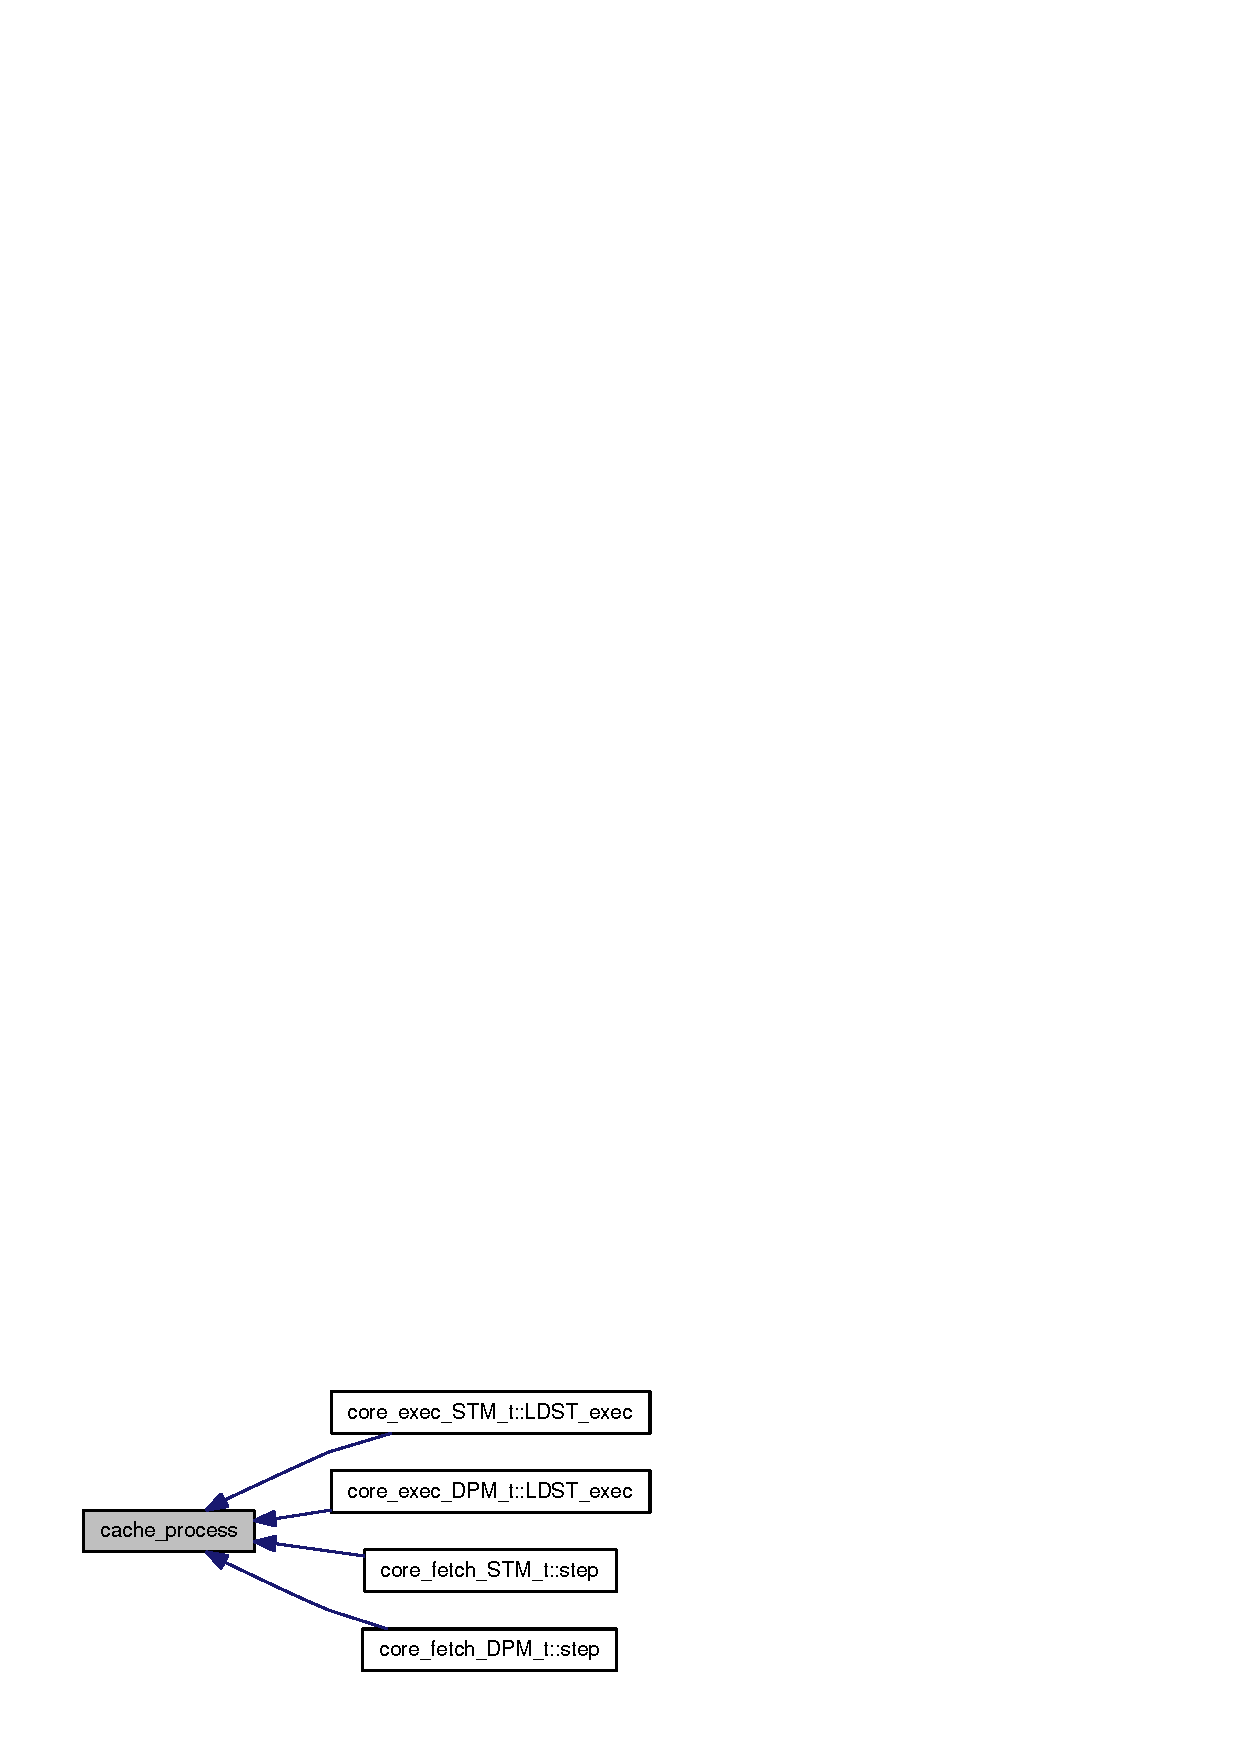
\includegraphics[width=158pt]{zesto-cache_8h_93ce14ef87e7565964216ea27d912147_icgraph}
\end{center}
\end{figure}
\index{zesto-cache.h@{zesto-cache.h}!cache\_\-process\_\-llc@{cache\_\-process\_\-llc}}
\index{cache\_\-process\_\-llc@{cache\_\-process\_\-llc}!zesto-cache.h@{zesto-cache.h}}
\subsubsection[{cache\_\-process\_\-llc}]{\setlength{\rightskip}{0pt plus 5cm}void cache\_\-process\_\-llc (struct {\bf cache\_\-t} $\ast$const  {\em cp})}\label{zesto-cache_8h_7b2967a29a17913e313fceec0d9dbd4c}




Definition at line 1422 of file config/zesto-llc.cpp.

References cache\_\-action\_\-t::action\_\-id, cache\_\-t::cache\_\-t::PFF\_\-t::addr, prefetch\_\-buffer\_\-t::addr, cache\_\-t::addr\_\-shift, cache\_\-t::allocate\_\-policy, cache\_\-t::bank\_\-mask, cache\_\-t::banks, BIG\_\-LATENCY, bus\_\-free(), bus\_\-use(), cache\_\-assert, cache\_\-fill\_\-llc(), cache\_\-fillable\_\-llc(), cache\_\-get\_\-evictee\_\-llc(), cache\_\-heap\_\-remove(), cache\_\-insert\_\-block\_\-llc(), cache\_\-invalidate(), cache\_\-is\_\-hit\_\-llc(), cache\_\-peek\_\-llc(), CACHE\_\-PREFETCH, CACHE\_\-READ, CACHE\_\-STAT, CACHE\_\-WRITE, CACHE\_\-WRITEBACK, cache\_\-action\_\-t::cb, cache\_\-t::check\_\-for\_\-fill\_\-work, cache\_\-t::check\_\-for\_\-MSHR\_\-fill\_\-work, cache\_\-t::check\_\-for\_\-MSHR\_\-work, cache\_\-t::check\_\-for\_\-pipe\_\-work, cache\_\-t::check\_\-for\_\-WBB\_\-work, cache\_\-t::check\_\-for\_\-work, cache\_\-action\_\-t::cmd, cache\_\-t::cache\_\-t::PFF\_\-t::core, cache\_\-line\_\-t::core, cache\_\-t::core, cache\_\-action\_\-t::core, cache\_\-t::core\_\-lookups, cache\_\-t::core\_\-misses, cache\_\-line\_\-t::dirty, uncore\_\-t::enqueuable(), uncore\_\-t::enqueue(), fatal(), fill\_\-arrived(), fill\_\-heap\_\-remove(), cache\_\-t::fill\_\-num, cache\_\-t::fill\_\-pipe, cache\_\-action\_\-t::get\_\-action\_\-id, GET\_\-MSHR\_\-BANK, cache\_\-t::latency, cache\_\-t::linesize, uncore\_\-t::LLC, cache\_\-t::load\_\-lookups, cache\_\-t::load\_\-misses, prefetch\_\-t::lookup(), cache\_\-action\_\-t::miss\_\-cb, cache\_\-action\_\-t::miss\_\-cb\_\-invoked, modinc(), cache\_\-t::MSHR, MSHR\_\-allocate(), MSHR\_\-available(), cache\_\-action\_\-t::MSHR\_\-bank, cache\_\-t::MSHR\_\-banks, cache\_\-t::MSHR\_\-full\_\-cycles, cache\_\-action\_\-t::MSHR\_\-index, cache\_\-action\_\-t::MSHR\_\-linked, cache\_\-t::MSHR\_\-mask, cache\_\-t::MSHR\_\-occupancy, cache\_\-t::MSHR\_\-size, cache\_\-t::name, prefetch\_\-buffer\_\-t::next, cache\_\-t::next\_\-bus, cache\_\-t::next\_\-level, NO\_\-MSHR, cache\_\-t::num\_\-prefetchers, cache\_\-action\_\-t::op, cache\_\-action\_\-t::paddr, PAGE\_\-SIZE, cache\_\-t::cache\_\-t::PFF\_\-t::PC, cache\_\-t::PF\_\-buffer, cache\_\-t::PF\_\-filter, cache\_\-t::PFF, cache\_\-t::PFF\_\-head, cache\_\-t::PFF\_\-num, cache\_\-t::PFF\_\-size, cache\_\-t::PFF\_\-tail, cache\_\-t::pipe, cache\_\-t::pipe\_\-num, prefetch\_\-filter\_\-lookup(), prefetch\_\-filter\_\-update(), cache\_\-t::prefetch\_\-lookups, cache\_\-t::prefetch\_\-misses, cache\_\-t::prefetch\_\-on\_\-miss, cache\_\-line\_\-t::prefetch\_\-used, cache\_\-t::prefetch\_\-useful\_\-insertions, cache\_\-line\_\-t::prefetched, cache\_\-t::prefetcher, cache\_\-action\_\-t::prev\_\-cp, cache\_\-t::prev\_\-level, sim\_\-cycle, cache\_\-t::start\_\-point, cache\_\-t::stat, cache\_\-t::store\_\-lookups, cache\_\-t::store\_\-misses, cache\_\-line\_\-t::tag, TICK\_\-T\_\-MAX, cache\_\-action\_\-t::translated\_\-cb, cache\_\-t::uncore, cache\_\-line\_\-t::valid, cache\_\-line\_\-t::victim, cache\_\-t::WBB, WBB\_\-available(), cache\_\-t::WBB\_\-combines, cache\_\-t::WBB\_\-full\_\-cycles, cache\_\-t::WBB\_\-head, cache\_\-t::WBB\_\-hits, WBB\_\-insert(), cache\_\-t::WBB\_\-num, cache\_\-t::WBB\_\-occupancy, cache\_\-t::WBB\_\-size, cache\_\-t::WBB\_\-victim\_\-hits, cache\_\-action\_\-t::when\_\-enqueued, cache\_\-action\_\-t::when\_\-returned, cache\_\-action\_\-t::when\_\-started, WRITE\_\-ALLOC, WRITE\_\-BACK, cache\_\-t::write\_\-combining, cache\_\-t::write\_\-policy, WRITE\_\-THROUGH, cache\_\-t::writeback\_\-lookups, and cache\_\-t::writeback\_\-misses.\index{zesto-cache.h@{zesto-cache.h}!cache\_\-reg\_\-stats@{cache\_\-reg\_\-stats}}
\index{cache\_\-reg\_\-stats@{cache\_\-reg\_\-stats}!zesto-cache.h@{zesto-cache.h}}
\subsubsection[{cache\_\-reg\_\-stats}]{\setlength{\rightskip}{0pt plus 5cm}void cache\_\-reg\_\-stats (struct {\bf stat\_\-sdb\_\-t} $\ast$const  {\em sdb}, \/  const struct {\bf core\_\-t} $\ast$const  {\em core}, \/  struct {\bf cache\_\-t} $\ast$const  {\em cp})}\label{zesto-cache_8h_80141f1bc8f06e0805162cdd6936c5d8}




Definition at line 280 of file config/zesto-cache.cpp.

References CACHE\_\-READWRITE, core\_\-t::current\_\-thread, fatal(), thread\_\-t::id, cache\_\-t::load\_\-lookups, cache\_\-t::load\_\-misses, cache\_\-t::MSHR\_\-combos, cache\_\-t::MSHR\_\-full\_\-cycles, cache\_\-t::MSHR\_\-occupancy, cache\_\-t::name, cache\_\-t::num\_\-prefetchers, cache\_\-t::prefetch\_\-insertions, cache\_\-t::prefetch\_\-lookups, cache\_\-t::prefetch\_\-misses, cache\_\-t::prefetch\_\-useful\_\-insertions, cache\_\-t::prefetcher, cache\_\-t::read\_\-only, prefetch\_\-t::reg\_\-stats(), cache\_\-t::stat, stat\_\-reg\_\-counter, stat\_\-reg\_\-formula(), cache\_\-t::store\_\-lookups, cache\_\-t::store\_\-misses, cache\_\-t::WBB\_\-combines, cache\_\-t::WBB\_\-full\_\-cycles, cache\_\-t::WBB\_\-hits, cache\_\-t::WBB\_\-insertions, cache\_\-t::WBB\_\-occupancy, cache\_\-t::WBB\_\-victim\_\-hits, cache\_\-t::WBB\_\-victim\_\-insertions, cache\_\-t::writeback\_\-lookups, and cache\_\-t::writeback\_\-misses.

Referenced by core\_\-fetch\_\-STM\_\-t::reg\_\-stats(), core\_\-fetch\_\-DPM\_\-t::reg\_\-stats(), core\_\-exec\_\-STM\_\-t::reg\_\-stats(), and core\_\-exec\_\-DPM\_\-t::reg\_\-stats().

Here is the caller graph for this function:\nopagebreak
\begin{figure}[H]
\begin{center}
\leavevmode
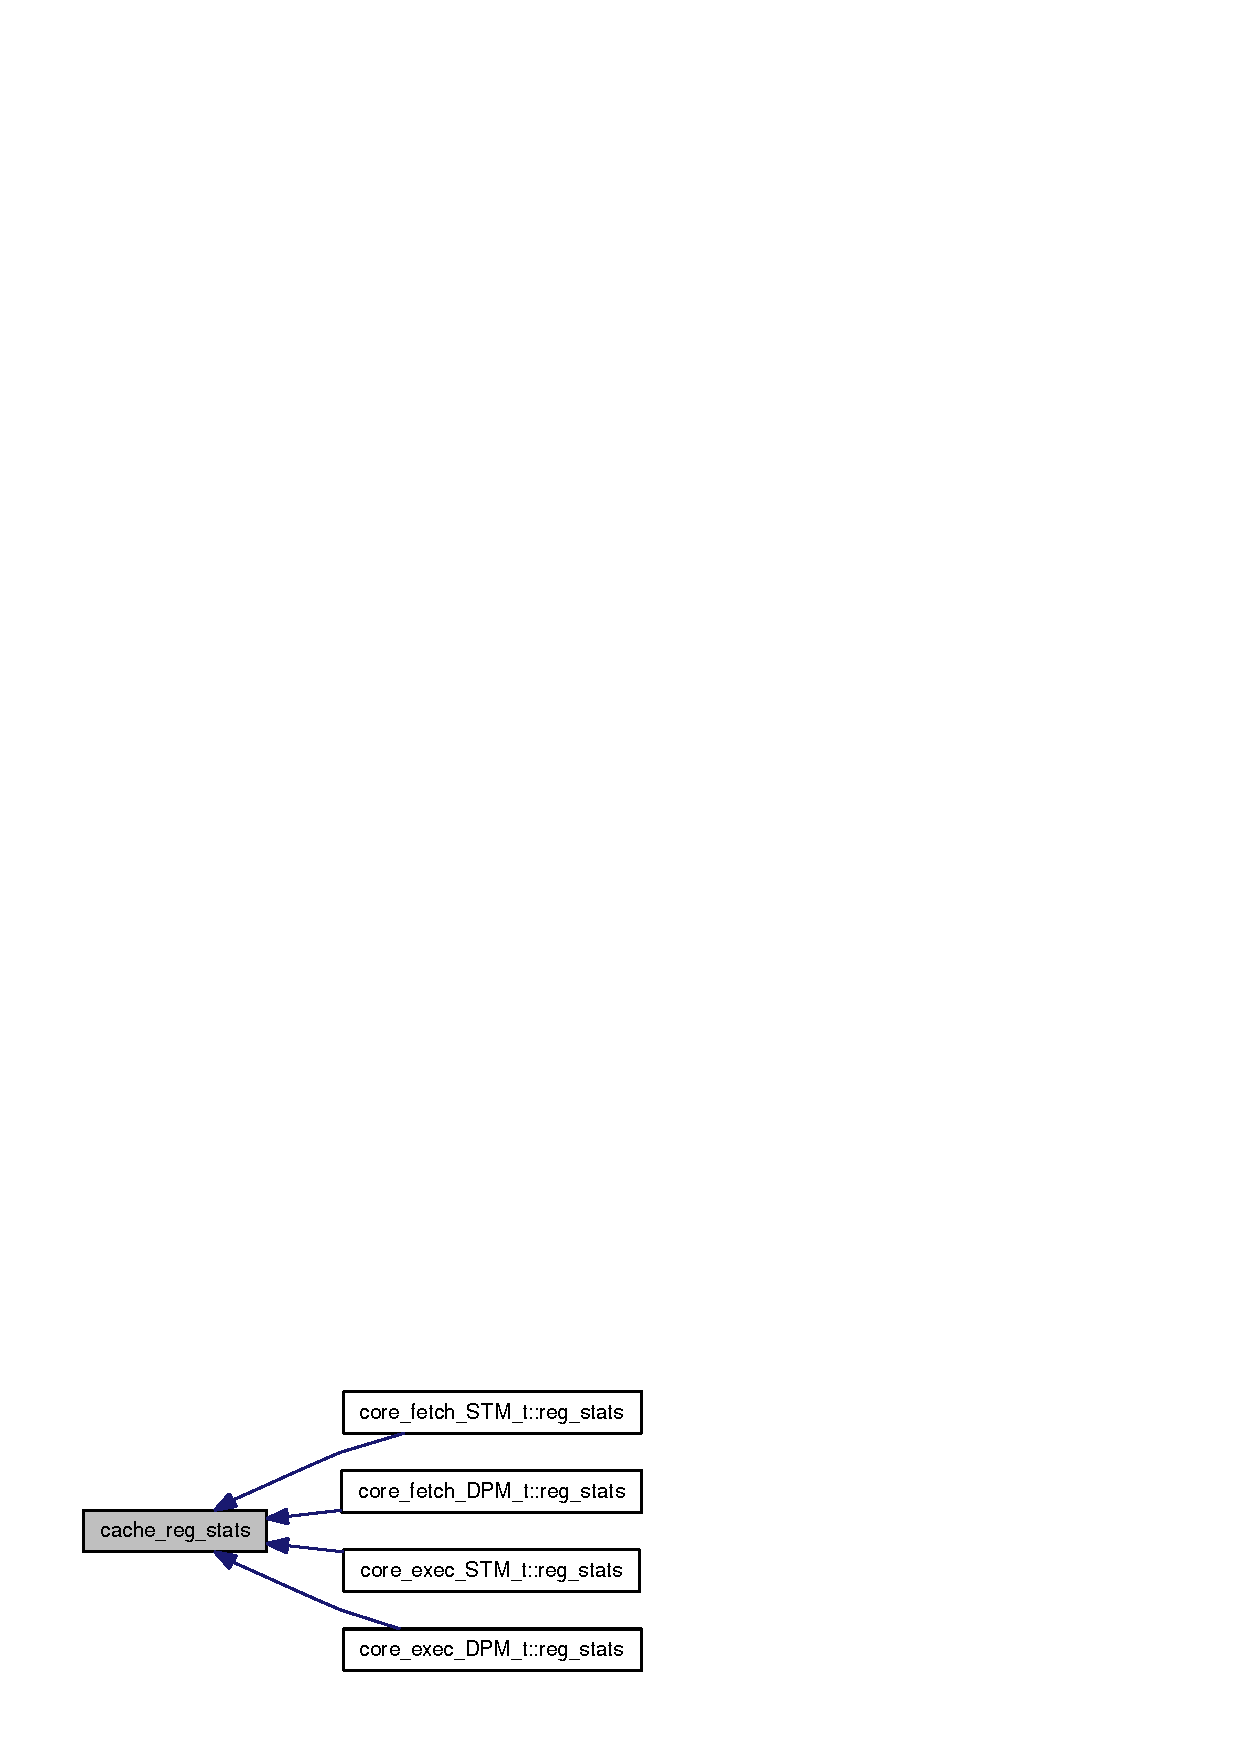
\includegraphics[width=156pt]{zesto-cache_8h_80141f1bc8f06e0805162cdd6936c5d8_icgraph}
\end{center}
\end{figure}
\index{zesto-cache.h@{zesto-cache.h}!cache\_\-reset\_\-stats@{cache\_\-reset\_\-stats}}
\index{cache\_\-reset\_\-stats@{cache\_\-reset\_\-stats}!zesto-cache.h@{zesto-cache.h}}
\subsubsection[{cache\_\-reset\_\-stats}]{\setlength{\rightskip}{0pt plus 5cm}void cache\_\-reset\_\-stats (struct {\bf cache\_\-t} $\ast$const  {\em cp})}\label{zesto-cache_8h_aff01697c94f19565dfd6d631bf4bf76}




Definition at line 515 of file config/zesto-cache.cpp.

References cache\_\-t::core\_\-lookups, cache\_\-t::core\_\-misses, memzero(), num\_\-threads, and cache\_\-t::stat.

Referenced by emergency\_\-recovery(), and sim\_\-fastfwd().

Here is the caller graph for this function:\nopagebreak
\begin{figure}[H]
\begin{center}
\leavevmode
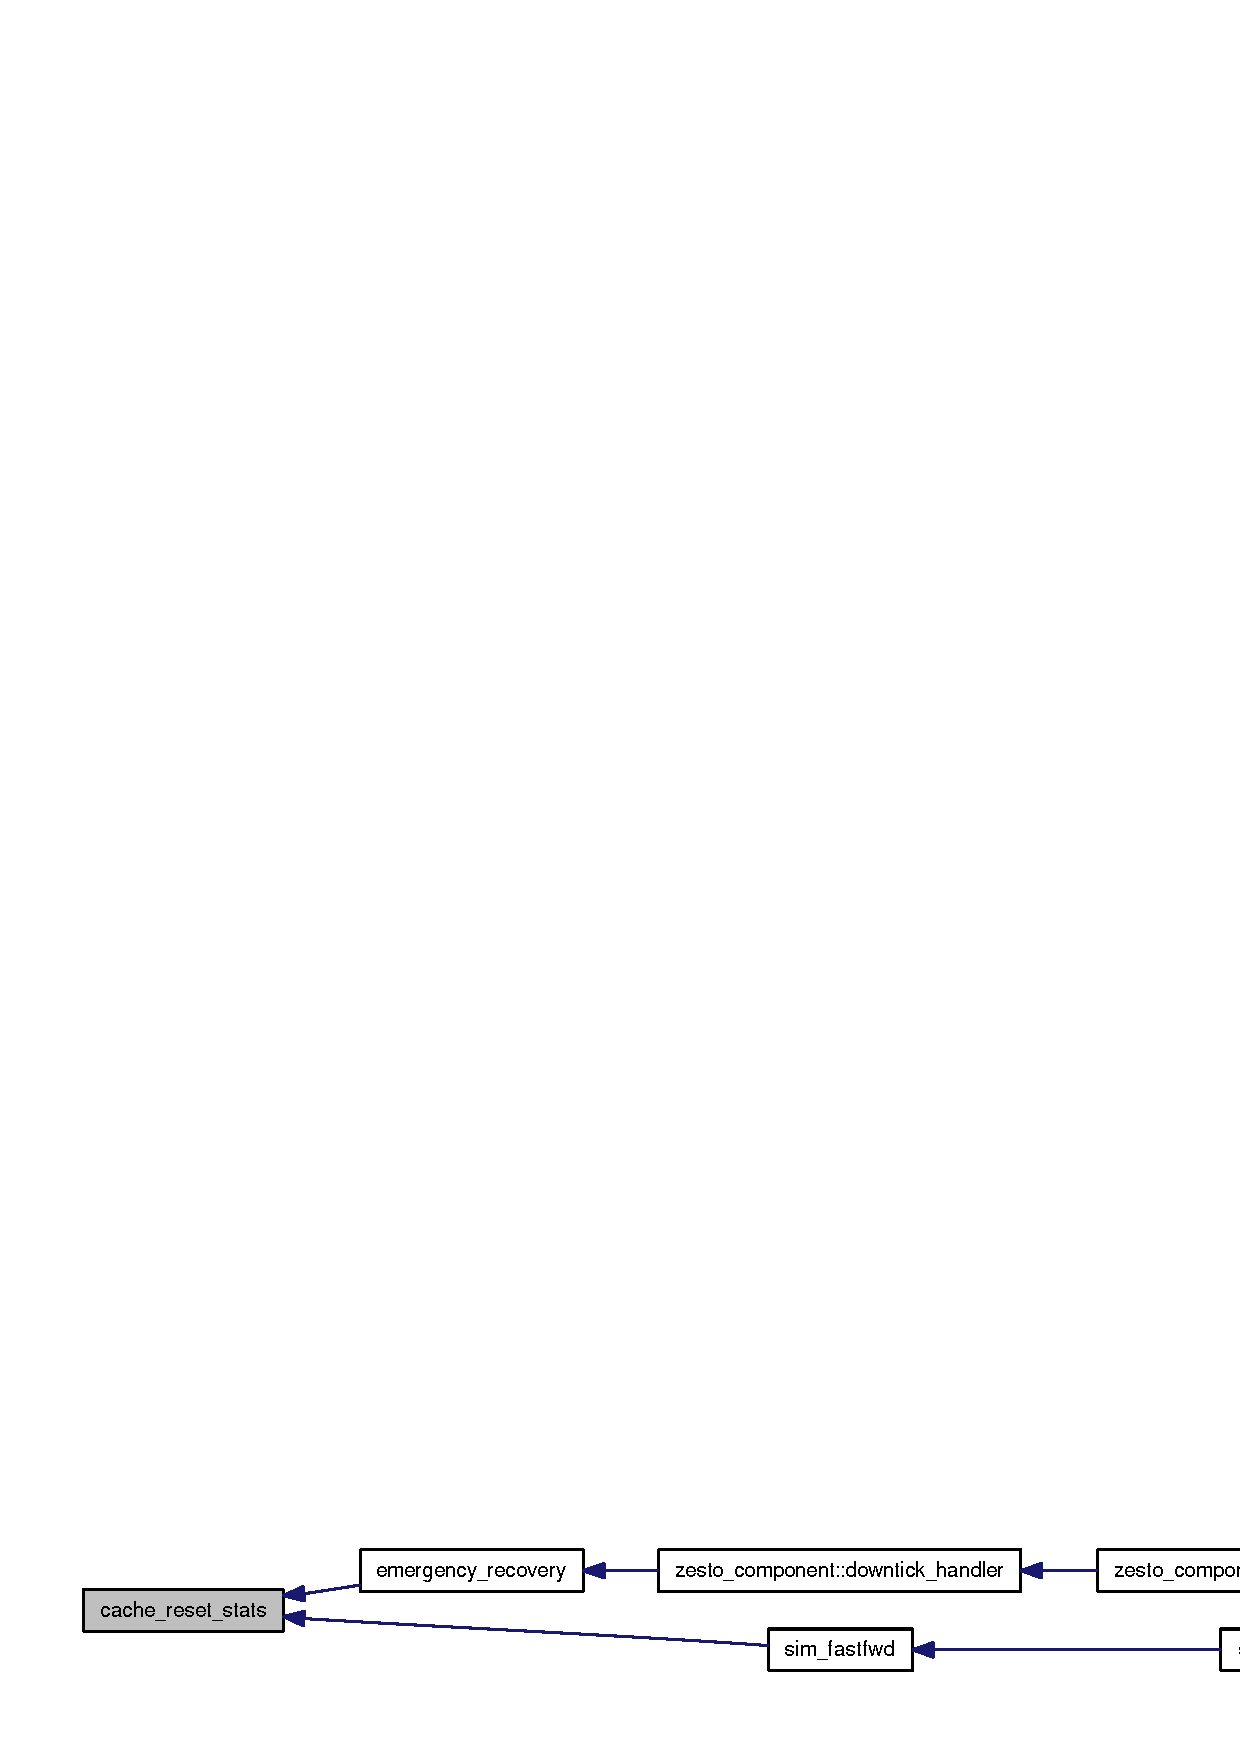
\includegraphics[width=391pt]{zesto-cache_8h_aff01697c94f19565dfd6d631bf4bf76_icgraph}
\end{center}
\end{figure}
\index{zesto-cache.h@{zesto-cache.h}!fill\_\-arrived@{fill\_\-arrived}}
\index{fill\_\-arrived@{fill\_\-arrived}!zesto-cache.h@{zesto-cache.h}}
\subsubsection[{fill\_\-arrived}]{\setlength{\rightskip}{0pt plus 5cm}void fill\_\-arrived (struct {\bf cache\_\-t} $\ast$const  {\em cp}, \/  const int {\em MSHR\_\-bank}, \/  const int {\em MSHR\_\-index})}\label{zesto-cache_8h_4d5f99649851ca3db130a4a6228a1f35}




Definition at line 1333 of file config/zesto-cache.cpp.

References cache\_\-assert, cache\_\-action\_\-t::cb, cache\_\-t::check\_\-for\_\-MSHR\_\-fill\_\-work, cache\_\-t::check\_\-for\_\-work, cache\_\-t::MSHR, cache\_\-action\_\-t::MSHR\_\-link, cache\_\-action\_\-t::MSHR\_\-linked, sim\_\-cycle, TICK\_\-T\_\-MAX, and cache\_\-action\_\-t::when\_\-returned.

Referenced by cache\_\-process(), and cache\_\-process\_\-llc().

Here is the caller graph for this function:\nopagebreak
\begin{figure}[H]
\begin{center}
\leavevmode
\includegraphics[width=214pt]{zesto-cache_8h_4d5f99649851ca3db130a4a6228a1f35_icgraph}
\end{center}
\end{figure}
\index{zesto-cache.h@{zesto-cache.h}!fill\_\-arrived\_\-llc@{fill\_\-arrived\_\-llc}}
\index{fill\_\-arrived\_\-llc@{fill\_\-arrived\_\-llc}!zesto-cache.h@{zesto-cache.h}}
\subsubsection[{fill\_\-arrived\_\-llc}]{\setlength{\rightskip}{0pt plus 5cm}void fill\_\-arrived\_\-llc (struct {\bf cache\_\-t} $\ast$const  {\em cp}, \/  unsigned long long int {\em address})}\label{zesto-cache_8h_f1f903df28f067bfd63f3145c04a5870}




Definition at line 1245 of file config/zesto-llc.cpp.

References cache\_\-t::addr\_\-shift, cache\_\-action\_\-t::cb, cache\_\-t::check\_\-for\_\-MSHR\_\-fill\_\-work, cache\_\-t::check\_\-for\_\-work, cache\_\-t::MSHR, cache\_\-t::MSHR\_\-banks, cache\_\-action\_\-t::MSHR\_\-link, cache\_\-action\_\-t::MSHR\_\-linked, cache\_\-t::MSHR\_\-mask, cache\_\-t::MSHR\_\-size, cache\_\-action\_\-t::paddr, sim\_\-cycle, and cache\_\-action\_\-t::when\_\-returned.\index{zesto-cache.h@{zesto-cache.h}!LLC\_\-reg\_\-stats@{LLC\_\-reg\_\-stats}}
\index{LLC\_\-reg\_\-stats@{LLC\_\-reg\_\-stats}!zesto-cache.h@{zesto-cache.h}}
\subsubsection[{LLC\_\-reg\_\-stats}]{\setlength{\rightskip}{0pt plus 5cm}void LLC\_\-reg\_\-stats (struct {\bf stat\_\-sdb\_\-t} $\ast$const  {\em sdb}, \/  struct {\bf cache\_\-t} $\ast$const  {\em cp})}\label{zesto-cache_8h_0a1aa47236ccba0a1d5e5818052a830d}




Definition at line 281 of file config/zesto-llc.cpp.

References CACHE\_\-READWRITE, uncore\_\-t::core, cache\_\-t::core\_\-lookups, cache\_\-t::core\_\-misses, core\_\-t::id, cache\_\-t::load\_\-lookups, cache\_\-t::load\_\-misses, cache\_\-t::MSHR\_\-combos, cache\_\-t::MSHR\_\-full\_\-cycles, cache\_\-t::MSHR\_\-occupancy, cache\_\-t::name, NetworkComponent::node\_\-ip, uncore\_\-t::num\_\-cores, cache\_\-t::num\_\-prefetchers, num\_\-threads, cache\_\-t::prefetch\_\-insertions, cache\_\-t::prefetch\_\-lookups, cache\_\-t::prefetch\_\-misses, cache\_\-t::prefetch\_\-useful\_\-insertions, cache\_\-t::prefetcher, cache\_\-t::read\_\-only, prefetch\_\-t::reg\_\-stats(), cache\_\-t::stat, stat\_\-reg\_\-counter, stat\_\-reg\_\-formula(), cache\_\-t::store\_\-lookups, cache\_\-t::store\_\-misses, cache\_\-t::uncore, cache\_\-t::WBB\_\-combines, cache\_\-t::WBB\_\-full\_\-cycles, cache\_\-t::WBB\_\-hits, cache\_\-t::WBB\_\-insertions, cache\_\-t::WBB\_\-occupancy, cache\_\-t::WBB\_\-victim\_\-hits, cache\_\-t::WBB\_\-victim\_\-insertions, cache\_\-t::writeback\_\-lookups, and cache\_\-t::writeback\_\-misses.\index{zesto-cache.h@{zesto-cache.h}!prefetch\_\-buffer\_\-create@{prefetch\_\-buffer\_\-create}}
\index{prefetch\_\-buffer\_\-create@{prefetch\_\-buffer\_\-create}!zesto-cache.h@{zesto-cache.h}}
\subsubsection[{prefetch\_\-buffer\_\-create}]{\setlength{\rightskip}{0pt plus 5cm}void prefetch\_\-buffer\_\-create (struct {\bf cache\_\-t} $\ast$const  {\em cp}, \/  const int {\em num\_\-entries})}\label{zesto-cache_8h_16dacff1f1e08b2a7fe82d35f3733f91}




Definition at line 531 of file config/zesto-cache.cpp.

References prefetch\_\-buffer\_\-t::addr, fatal(), prefetch\_\-buffer\_\-t::next, cache\_\-t::PF\_\-buffer, and cache\_\-t::PF\_\-buffer\_\-size.

Referenced by core\_\-exec\_\-DPM\_\-t::core\_\-exec\_\-DPM\_\-t(), core\_\-fetch\_\-DPM\_\-t::core\_\-fetch\_\-DPM\_\-t(), and uncore\_\-t::uncore\_\-t().

Here is the caller graph for this function:\nopagebreak
\begin{figure}[H]
\begin{center}
\leavevmode
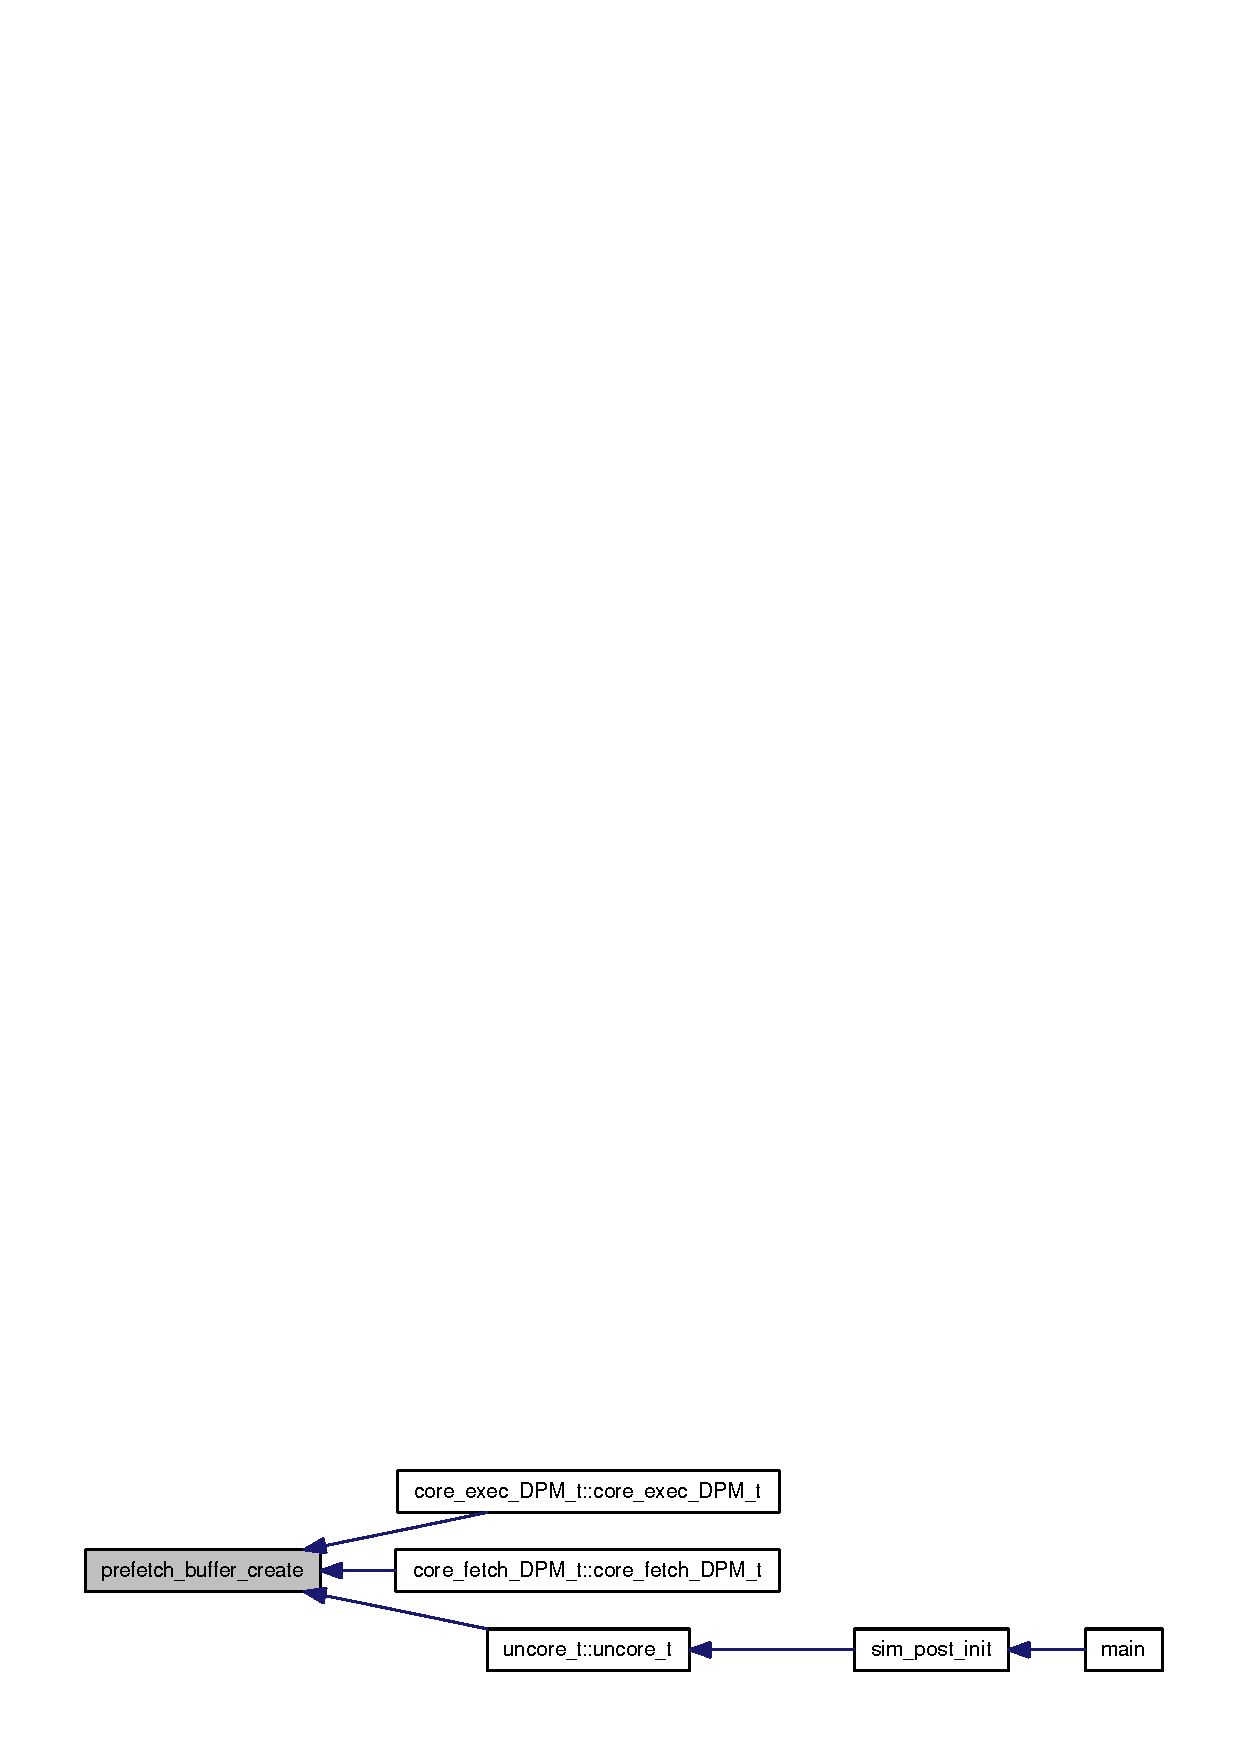
\includegraphics[width=281pt]{zesto-cache_8h_16dacff1f1e08b2a7fe82d35f3733f91_icgraph}
\end{center}
\end{figure}
\index{zesto-cache.h@{zesto-cache.h}!prefetch\_\-core\_\-caches@{prefetch\_\-core\_\-caches}}
\index{prefetch\_\-core\_\-caches@{prefetch\_\-core\_\-caches}!zesto-cache.h@{zesto-cache.h}}
\subsubsection[{prefetch\_\-core\_\-caches}]{\setlength{\rightskip}{0pt plus 5cm}void prefetch\_\-core\_\-caches (struct {\bf core\_\-t} $\ast$const  {\em core})}\label{zesto-cache_8h_3f3ef48df254425f422f6cf5de128ade}




Definition at line 2395 of file config/zesto-cache.cpp.

References cache\_\-prefetch(), core\_\-t::core\_\-t::core\_\-memory\_\-t::DL1, core\_\-t::core\_\-t::core\_\-memory\_\-t::DL2, core\_\-t::core\_\-t::core\_\-memory\_\-t::IL1, and core\_\-t::memory.

Referenced by zesto\_\-component::downtick\_\-handler().

Here is the caller graph for this function:\nopagebreak
\begin{figure}[H]
\begin{center}
\leavevmode
\includegraphics[width=327pt]{zesto-cache_8h_3f3ef48df254425f422f6cf5de128ade_icgraph}
\end{center}
\end{figure}
\index{zesto-cache.h@{zesto-cache.h}!prefetch\_\-filter\_\-create@{prefetch\_\-filter\_\-create}}
\index{prefetch\_\-filter\_\-create@{prefetch\_\-filter\_\-create}!zesto-cache.h@{zesto-cache.h}}
\subsubsection[{prefetch\_\-filter\_\-create}]{\setlength{\rightskip}{0pt plus 5cm}void prefetch\_\-filter\_\-create (struct {\bf cache\_\-t} $\ast$const  {\em cp}, \/  const int {\em num\_\-entries}, \/  const int {\em reset\_\-interval})}\label{zesto-cache_8h_81be4d7fbc22a3d9f3fcaa52715c22e9}




Definition at line 552 of file config/zesto-cache.cpp.

References fatal(), prefetch\_\-filter\_\-t::mask, prefetch\_\-filter\_\-t::num\_\-entries, cache\_\-t::PF\_\-filter, prefetch\_\-filter\_\-t::reset\_\-interval, and prefetch\_\-filter\_\-t::table.

Referenced by core\_\-exec\_\-DPM\_\-t::core\_\-exec\_\-DPM\_\-t(), core\_\-fetch\_\-DPM\_\-t::core\_\-fetch\_\-DPM\_\-t(), and uncore\_\-t::uncore\_\-t().

Here is the caller graph for this function:\nopagebreak
\begin{figure}[H]
\begin{center}
\leavevmode
\includegraphics[width=278pt]{zesto-cache_8h_81be4d7fbc22a3d9f3fcaa52715c22e9_icgraph}
\end{center}
\end{figure}
\index{zesto-cache.h@{zesto-cache.h}!prefetch\_\-LLC@{prefetch\_\-LLC}}
\index{prefetch\_\-LLC@{prefetch\_\-LLC}!zesto-cache.h@{zesto-cache.h}}
\subsubsection[{prefetch\_\-LLC}]{\setlength{\rightskip}{0pt plus 5cm}void prefetch\_\-LLC (struct {\bf uncore\_\-t} $\ast$const  {\em uncore})}\label{zesto-cache_8h_8ed5f90d7b07bddefbf6736b13da8eb2}




Definition at line 2229 of file config/zesto-llc.cpp.

References cache\_\-prefetch\_\-llc(), and uncore\_\-t::LLC.\index{zesto-cache.h@{zesto-cache.h}!step\_\-core\_\-PF\_\-controllers@{step\_\-core\_\-PF\_\-controllers}}
\index{step\_\-core\_\-PF\_\-controllers@{step\_\-core\_\-PF\_\-controllers}!zesto-cache.h@{zesto-cache.h}}
\subsubsection[{step\_\-core\_\-PF\_\-controllers}]{\setlength{\rightskip}{0pt plus 5cm}void step\_\-core\_\-PF\_\-controllers (struct {\bf core\_\-t} $\ast$const  {\em core})}\label{zesto-cache_8h_66309167ab5b4ca25ad2bfbf94b0126b}




Definition at line 2387 of file config/zesto-cache.cpp.

References core\_\-t::core\_\-t::core\_\-memory\_\-t::DL1, core\_\-t::core\_\-t::core\_\-memory\_\-t::DL2, core\_\-t::core\_\-t::core\_\-memory\_\-t::IL1, core\_\-t::memory, and prefetch\_\-controller\_\-update().

Referenced by zesto\_\-component::downtick\_\-handler().

Here is the caller graph for this function:\nopagebreak
\begin{figure}[H]
\begin{center}
\leavevmode
\includegraphics[width=335pt]{zesto-cache_8h_66309167ab5b4ca25ad2bfbf94b0126b_icgraph}
\end{center}
\end{figure}
\index{zesto-cache.h@{zesto-cache.h}!step\_\-LLC\_\-PF\_\-controller@{step\_\-LLC\_\-PF\_\-controller}}
\index{step\_\-LLC\_\-PF\_\-controller@{step\_\-LLC\_\-PF\_\-controller}!zesto-cache.h@{zesto-cache.h}}
\subsubsection[{step\_\-LLC\_\-PF\_\-controller}]{\setlength{\rightskip}{0pt plus 5cm}void step\_\-LLC\_\-PF\_\-controller (struct {\bf uncore\_\-t} $\ast$const  {\em uncore})}\label{zesto-cache_8h_65086cfd5f54ff7a76a41587c8f6a01e}




Definition at line 2223 of file config/zesto-llc.cpp.

References uncore\_\-t::LLC, and prefetch\_\-controller\_\-update\_\-llc().